% Options for packages loaded elsewhere
\PassOptionsToPackage{unicode}{hyperref}
\PassOptionsToPackage{hyphens}{url}
\PassOptionsToPackage{dvipsnames,svgnames,x11names}{xcolor}
%
\documentclass[
  letterpaper,
  DIV=11,
  numbers=noendperiod]{scrartcl}

\usepackage{amsmath,amssymb}
\usepackage{iftex}
\ifPDFTeX
  \usepackage[T1]{fontenc}
  \usepackage[utf8]{inputenc}
  \usepackage{textcomp} % provide euro and other symbols
\else % if luatex or xetex
  \usepackage{unicode-math}
  \defaultfontfeatures{Scale=MatchLowercase}
  \defaultfontfeatures[\rmfamily]{Ligatures=TeX,Scale=1}
\fi
\usepackage{lmodern}
\ifPDFTeX\else  
    % xetex/luatex font selection
\fi
% Use upquote if available, for straight quotes in verbatim environments
\IfFileExists{upquote.sty}{\usepackage{upquote}}{}
\IfFileExists{microtype.sty}{% use microtype if available
  \usepackage[]{microtype}
  \UseMicrotypeSet[protrusion]{basicmath} % disable protrusion for tt fonts
}{}
\makeatletter
\@ifundefined{KOMAClassName}{% if non-KOMA class
  \IfFileExists{parskip.sty}{%
    \usepackage{parskip}
  }{% else
    \setlength{\parindent}{0pt}
    \setlength{\parskip}{6pt plus 2pt minus 1pt}}
}{% if KOMA class
  \KOMAoptions{parskip=half}}
\makeatother
\usepackage{xcolor}
\setlength{\emergencystretch}{3em} % prevent overfull lines
\setcounter{secnumdepth}{-\maxdimen} % remove section numbering
% Make \paragraph and \subparagraph free-standing
\makeatletter
\ifx\paragraph\undefined\else
  \let\oldparagraph\paragraph
  \renewcommand{\paragraph}{
    \@ifstar
      \xxxParagraphStar
      \xxxParagraphNoStar
  }
  \newcommand{\xxxParagraphStar}[1]{\oldparagraph*{#1}\mbox{}}
  \newcommand{\xxxParagraphNoStar}[1]{\oldparagraph{#1}\mbox{}}
\fi
\ifx\subparagraph\undefined\else
  \let\oldsubparagraph\subparagraph
  \renewcommand{\subparagraph}{
    \@ifstar
      \xxxSubParagraphStar
      \xxxSubParagraphNoStar
  }
  \newcommand{\xxxSubParagraphStar}[1]{\oldsubparagraph*{#1}\mbox{}}
  \newcommand{\xxxSubParagraphNoStar}[1]{\oldsubparagraph{#1}\mbox{}}
\fi
\makeatother

\usepackage{color}
\usepackage{fancyvrb}
\newcommand{\VerbBar}{|}
\newcommand{\VERB}{\Verb[commandchars=\\\{\}]}
\DefineVerbatimEnvironment{Highlighting}{Verbatim}{commandchars=\\\{\}}
% Add ',fontsize=\small' for more characters per line
\usepackage{framed}
\definecolor{shadecolor}{RGB}{241,243,245}
\newenvironment{Shaded}{\begin{snugshade}}{\end{snugshade}}
\newcommand{\AlertTok}[1]{\textcolor[rgb]{0.68,0.00,0.00}{#1}}
\newcommand{\AnnotationTok}[1]{\textcolor[rgb]{0.37,0.37,0.37}{#1}}
\newcommand{\AttributeTok}[1]{\textcolor[rgb]{0.40,0.45,0.13}{#1}}
\newcommand{\BaseNTok}[1]{\textcolor[rgb]{0.68,0.00,0.00}{#1}}
\newcommand{\BuiltInTok}[1]{\textcolor[rgb]{0.00,0.23,0.31}{#1}}
\newcommand{\CharTok}[1]{\textcolor[rgb]{0.13,0.47,0.30}{#1}}
\newcommand{\CommentTok}[1]{\textcolor[rgb]{0.37,0.37,0.37}{#1}}
\newcommand{\CommentVarTok}[1]{\textcolor[rgb]{0.37,0.37,0.37}{\textit{#1}}}
\newcommand{\ConstantTok}[1]{\textcolor[rgb]{0.56,0.35,0.01}{#1}}
\newcommand{\ControlFlowTok}[1]{\textcolor[rgb]{0.00,0.23,0.31}{\textbf{#1}}}
\newcommand{\DataTypeTok}[1]{\textcolor[rgb]{0.68,0.00,0.00}{#1}}
\newcommand{\DecValTok}[1]{\textcolor[rgb]{0.68,0.00,0.00}{#1}}
\newcommand{\DocumentationTok}[1]{\textcolor[rgb]{0.37,0.37,0.37}{\textit{#1}}}
\newcommand{\ErrorTok}[1]{\textcolor[rgb]{0.68,0.00,0.00}{#1}}
\newcommand{\ExtensionTok}[1]{\textcolor[rgb]{0.00,0.23,0.31}{#1}}
\newcommand{\FloatTok}[1]{\textcolor[rgb]{0.68,0.00,0.00}{#1}}
\newcommand{\FunctionTok}[1]{\textcolor[rgb]{0.28,0.35,0.67}{#1}}
\newcommand{\ImportTok}[1]{\textcolor[rgb]{0.00,0.46,0.62}{#1}}
\newcommand{\InformationTok}[1]{\textcolor[rgb]{0.37,0.37,0.37}{#1}}
\newcommand{\KeywordTok}[1]{\textcolor[rgb]{0.00,0.23,0.31}{\textbf{#1}}}
\newcommand{\NormalTok}[1]{\textcolor[rgb]{0.00,0.23,0.31}{#1}}
\newcommand{\OperatorTok}[1]{\textcolor[rgb]{0.37,0.37,0.37}{#1}}
\newcommand{\OtherTok}[1]{\textcolor[rgb]{0.00,0.23,0.31}{#1}}
\newcommand{\PreprocessorTok}[1]{\textcolor[rgb]{0.68,0.00,0.00}{#1}}
\newcommand{\RegionMarkerTok}[1]{\textcolor[rgb]{0.00,0.23,0.31}{#1}}
\newcommand{\SpecialCharTok}[1]{\textcolor[rgb]{0.37,0.37,0.37}{#1}}
\newcommand{\SpecialStringTok}[1]{\textcolor[rgb]{0.13,0.47,0.30}{#1}}
\newcommand{\StringTok}[1]{\textcolor[rgb]{0.13,0.47,0.30}{#1}}
\newcommand{\VariableTok}[1]{\textcolor[rgb]{0.07,0.07,0.07}{#1}}
\newcommand{\VerbatimStringTok}[1]{\textcolor[rgb]{0.13,0.47,0.30}{#1}}
\newcommand{\WarningTok}[1]{\textcolor[rgb]{0.37,0.37,0.37}{\textit{#1}}}

\providecommand{\tightlist}{%
  \setlength{\itemsep}{0pt}\setlength{\parskip}{0pt}}\usepackage{longtable,booktabs,array}
\usepackage{calc} % for calculating minipage widths
% Correct order of tables after \paragraph or \subparagraph
\usepackage{etoolbox}
\makeatletter
\patchcmd\longtable{\par}{\if@noskipsec\mbox{}\fi\par}{}{}
\makeatother
% Allow footnotes in longtable head/foot
\IfFileExists{footnotehyper.sty}{\usepackage{footnotehyper}}{\usepackage{footnote}}
\makesavenoteenv{longtable}
\usepackage{graphicx}
\makeatletter
\def\maxwidth{\ifdim\Gin@nat@width>\linewidth\linewidth\else\Gin@nat@width\fi}
\def\maxheight{\ifdim\Gin@nat@height>\textheight\textheight\else\Gin@nat@height\fi}
\makeatother
% Scale images if necessary, so that they will not overflow the page
% margins by default, and it is still possible to overwrite the defaults
% using explicit options in \includegraphics[width, height, ...]{}
\setkeys{Gin}{width=\maxwidth,height=\maxheight,keepaspectratio}
% Set default figure placement to htbp
\makeatletter
\def\fps@figure{htbp}
\makeatother

\usepackage{fvextra}
\DefineVerbatimEnvironment{Highlighting}{Verbatim}{breaklines,commandchars=\\\{\}}
\KOMAoption{captions}{tableheading}
\makeatletter
\@ifpackageloaded{caption}{}{\usepackage{caption}}
\AtBeginDocument{%
\ifdefined\contentsname
  \renewcommand*\contentsname{Table of contents}
\else
  \newcommand\contentsname{Table of contents}
\fi
\ifdefined\listfigurename
  \renewcommand*\listfigurename{List of Figures}
\else
  \newcommand\listfigurename{List of Figures}
\fi
\ifdefined\listtablename
  \renewcommand*\listtablename{List of Tables}
\else
  \newcommand\listtablename{List of Tables}
\fi
\ifdefined\figurename
  \renewcommand*\figurename{Figure}
\else
  \newcommand\figurename{Figure}
\fi
\ifdefined\tablename
  \renewcommand*\tablename{Table}
\else
  \newcommand\tablename{Table}
\fi
}
\@ifpackageloaded{float}{}{\usepackage{float}}
\floatstyle{ruled}
\@ifundefined{c@chapter}{\newfloat{codelisting}{h}{lop}}{\newfloat{codelisting}{h}{lop}[chapter]}
\floatname{codelisting}{Listing}
\newcommand*\listoflistings{\listof{codelisting}{List of Listings}}
\makeatother
\makeatletter
\makeatother
\makeatletter
\@ifpackageloaded{caption}{}{\usepackage{caption}}
\@ifpackageloaded{subcaption}{}{\usepackage{subcaption}}
\makeatother

\ifLuaTeX
  \usepackage{selnolig}  % disable illegal ligatures
\fi
\usepackage{bookmark}

\IfFileExists{xurl.sty}{\usepackage{xurl}}{} % add URL line breaks if available
\urlstyle{same} % disable monospaced font for URLs
\hypersetup{
  pdftitle={ps2\_answers},
  colorlinks=true,
  linkcolor={blue},
  filecolor={Maroon},
  citecolor={Blue},
  urlcolor={Blue},
  pdfcreator={LaTeX via pandoc}}


\title{ps2\_answers}
\author{}
\date{}

\begin{document}
\maketitle

\RecustomVerbatimEnvironment{verbatim}{Verbatim}{
  showspaces = false,
  showtabs = false,
  breaksymbolleft={},
  breaklines
}


\begin{enumerate}
\def\labelenumi{\arabic{enumi}.}
\tightlist
\item
  ``This submission is my work alone and complies with the 30538
  integrity policy.'' Add your initials to indicate your agreement:
  \emph{CT}
\item
  ``I have uploaded the names of anyone I worked with on the problem set
  \textbf{\href{https://docs.google.com/forms/d/1-zzHx762odGlpVWtgdIC55vqF-j3gqdAp6Pno1rIGK0/edit}{here}}''
  **\C\T** (1 point)
\item
  Late coins used this pset: **\textbackslash1** Late coins left after
  submission: \emph{2}
\end{enumerate}

Integrity statement: I used AI to help me debug and organize my code.

\begin{Shaded}
\begin{Highlighting}[]
\ImportTok{import}\NormalTok{ pandas }\ImportTok{as}\NormalTok{ pd}
\ImportTok{import}\NormalTok{ altair }\ImportTok{as}\NormalTok{ alt}
\NormalTok{alt.renderers.enable(}\StringTok{"png"}\NormalTok{)}
\ImportTok{import}\NormalTok{ time}
\ImportTok{from}\NormalTok{ vega\_datasets }\ImportTok{import}\NormalTok{ data }\ImportTok{as}\NormalTok{ vega\_data}
\ImportTok{import}\NormalTok{ warnings }
\NormalTok{warnings.filterwarnings(}\StringTok{\textquotesingle{}ignore\textquotesingle{}}\NormalTok{)}
\end{Highlighting}
\end{Shaded}

\subsubsection{Data cleaning continued (15
points)}\label{data-cleaning-continued-15-points}

Reading in one percent sample

\begin{Shaded}
\begin{Highlighting}[]
\CommentTok{\# Reading in file}
\NormalTok{file\_path }\OperatorTok{=} \VerbatimStringTok{r\textquotesingle{}C:\textbackslash{}Users\textbackslash{}clari\textbackslash{}OneDrive\textbackslash{}Documents\textbackslash{}Python II\textbackslash{}student30538\textbackslash{}problem\_sets\textbackslash{}ps2\textbackslash{}data\textbackslash{}parking\_tickets\_one\_percent.csv\textquotesingle{}}
\NormalTok{df }\OperatorTok{=}\NormalTok{ pd.read\_csv(file\_path)}
\end{Highlighting}
\end{Shaded}

\subsection{1.1}\label{section}

Function to create a 2 col dataframe (COl1 = variable name, col2 = num
of times the col is NA)

\begin{Shaded}
\begin{Highlighting}[]
\KeywordTok{def}\NormalTok{ count\_nas(df):}
\NormalTok{    na\_counts }\OperatorTok{=}\NormalTok{ df.isna().}\BuiltInTok{sum}\NormalTok{().reset\_index()}
\NormalTok{    na\_counts.columns }\OperatorTok{=}\NormalTok{ [}\StringTok{\textquotesingle{}Variable\textquotesingle{}}\NormalTok{, }\StringTok{\textquotesingle{}NA\_Count\textquotesingle{}}\NormalTok{]}
    \ControlFlowTok{return}\NormalTok{ na\_counts.set\_index(}\StringTok{\textquotesingle{}Variable\textquotesingle{}}\NormalTok{)}
\NormalTok{two\_col\_df }\OperatorTok{=}\NormalTok{ count\_nas(df)}

\BuiltInTok{print}\NormalTok{(two\_col\_df)}
\end{Highlighting}
\end{Shaded}

\begin{verbatim}
                       NA_Count
Variable                       
Unnamed: 0                    0
ticket_number                 0
issue_date                    0
violation_location            0
license_plate_number          0
license_plate_state          97
license_plate_type         2054
zipcode                   54115
violation_code                0
violation_description         0
unit                         29
unit_description              0
vehicle_make                  0
fine_level1_amount            0
fine_level2_amount            0
current_amount_due            0
total_payments                0
ticket_queue                  0
ticket_queue_date             0
notice_level              84068
hearing_disposition      259899
notice_number                 0
officer                       0
address                       0
\end{verbatim}

https://saturncloud.io/blog/how-to-count-the-number-of-missingnan-values-in-each-row-in-python-pandas/\#:\textasciitilde:text=(axis\%3D1)-,To\%20count\%20the\%20number\%20of\%20missing\%2FNaN\%20values\%20in\%20each,True\%20values\%20in\%20each\%20row.

\subsection{1.2}\label{section-1}

Three variables are missing much more frequently than the others. Why?
(Hint: look at some rows and read the data dictionary written by
ProPublica)

\begin{Shaded}
\begin{Highlighting}[]
\NormalTok{descending\_two\_col\_df }\OperatorTok{=}\NormalTok{ two\_col\_df.sort\_values(by}\OperatorTok{=}\StringTok{\textquotesingle{}NA\_Count\textquotesingle{}}\NormalTok{, ascending}\OperatorTok{=}\VariableTok{False}\NormalTok{)}
\BuiltInTok{print}\NormalTok{(descending\_two\_col\_df)}
\end{Highlighting}
\end{Shaded}

\begin{verbatim}
                       NA_Count
Variable                       
hearing_disposition      259899
notice_level              84068
zipcode                   54115
license_plate_type         2054
license_plate_state          97
unit                         29
Unnamed: 0                    0
fine_level2_amount            0
officer                       0
notice_number                 0
ticket_queue_date             0
ticket_queue                  0
total_payments                0
current_amount_due            0
vehicle_make                  0
fine_level1_amount            0
ticket_number                 0
unit_description              0
violation_description         0
violation_code                0
license_plate_number          0
violation_location            0
issue_date                    0
address                       0
\end{verbatim}

Hearing disposition (259899), notice \_level (84068), and zipcode(54115)
tend to have the most NA Values {[}EXPLAIN WHY{]}

\subsection{1.3}\label{section-2}

Through visual inspection: The old code is:0964125 The new code: 964125B

\begin{Shaded}
\begin{Highlighting}[]
\CommentTok{\# Filtering for anything that contains "NO STICKER"}
\NormalTok{filtered\_violations }\OperatorTok{=}\NormalTok{ df[df[}\StringTok{\textquotesingle{}violation\_description\textquotesingle{}}\NormalTok{].}\BuiltInTok{str}\NormalTok{.contains(}
    \StringTok{\textquotesingle{}NO CITY STICKER\textquotesingle{}}\NormalTok{)]}

\CommentTok{\# Get the unique violation codes}
\NormalTok{violation\_codes }\OperatorTok{=}\NormalTok{ filtered\_violations[}\StringTok{\textquotesingle{}violation\_code\textquotesingle{}}\NormalTok{].unique().tolist()}

\BuiltInTok{print}\NormalTok{(}\StringTok{"Violation codes for \textquotesingle{}NO CITY STICKER\textquotesingle{}:"}\NormalTok{)}
\BuiltInTok{print}\NormalTok{(violation\_codes)}
\end{Highlighting}
\end{Shaded}

\begin{verbatim}
Violation codes for 'NO CITY STICKER':
['0964125', '0976170', '0964125B', '0964125C']
\end{verbatim}

From this, I see that 0976170 is a different code number.

\subsection{1.4}\label{section-3}

\begin{Shaded}
\begin{Highlighting}[]
\CommentTok{\# New df filtered for violation codes for no sticker, retaining issue date, violation code, fine levels}
\NormalTok{violation\_fines }\OperatorTok{=}\NormalTok{ filtered\_violations[filtered\_violations[}\StringTok{\textquotesingle{}violation\_code\textquotesingle{}}\NormalTok{].isin(}
\NormalTok{    [}\StringTok{\textquotesingle{}0964125\textquotesingle{}}\NormalTok{, }\StringTok{\textquotesingle{}0964125B\textquotesingle{}}\NormalTok{, }\StringTok{\textquotesingle{}976170\textquotesingle{}}\NormalTok{])][[}\StringTok{\textquotesingle{}issue\_date\textquotesingle{}}\NormalTok{, }\StringTok{\textquotesingle{}violation\_code\textquotesingle{}}\NormalTok{, }\StringTok{\textquotesingle{}fine\_level1\_amount\textquotesingle{}}\NormalTok{, }\StringTok{\textquotesingle{}fine\_level2\_amount\textquotesingle{}}\NormalTok{]]}
\BuiltInTok{print}\NormalTok{(violation\_fines)}

\CommentTok{\# Putting it in descending order to check for new rate}
\NormalTok{violation\_fines\_descending }\OperatorTok{=}\NormalTok{ violation\_fines.sort\_values(}
\NormalTok{    by}\OperatorTok{=}\StringTok{\textquotesingle{}fine\_level1\_amount\textquotesingle{}}\NormalTok{, ascending}\OperatorTok{=}\VariableTok{False}\NormalTok{)}
\BuiltInTok{print}\NormalTok{(violation\_fines\_descending)}

\CommentTok{\# Putting it in ascending order to check for old rate}
\NormalTok{violation\_fines\_ascending }\OperatorTok{=}\NormalTok{ violation\_fines.sort\_values(}
\NormalTok{    by}\OperatorTok{=}\StringTok{\textquotesingle{}fine\_level1\_amount\textquotesingle{}}\NormalTok{)}
\BuiltInTok{print}\NormalTok{(violation\_fines\_ascending)}
\end{Highlighting}
\end{Shaded}

\begin{verbatim}
                 issue_date violation_code  fine_level1_amount  \
14      2007-01-01 10:51:00        0964125                 120   
29      2007-01-01 17:55:00        0964125                 120   
82      2007-01-02 10:20:00        0964125                 120   
97      2007-01-02 12:12:00        0964125                 120   
104     2007-01-02 13:39:00        0964125                 120   
...                     ...            ...                 ...   
287420  2018-05-14 08:53:00       0964125B                 200   
287440  2018-05-14 11:50:00       0964125B                 200   
287441  2018-05-14 12:09:00       0964125B                 200   
287450  2018-05-14 14:11:00       0964125B                 200   
287452  2018-05-14 14:30:00       0964125B                 200   

        fine_level2_amount  
14                     240  
29                     240  
82                     240  
97                     240  
104                    240  
...                    ...  
287420                 400  
287440                 400  
287441                 400  
287450                 400  
287452                 400  

[25004 rows x 4 columns]
                 issue_date violation_code  fine_level1_amount  \
157196  2012-11-15 19:01:00       0964125B                 200   
202661  2014-08-31 17:07:00       0964125B                 200   
202909  2014-09-04 08:21:00       0964125B                 200   
202901  2014-09-04 01:42:00       0964125B                 200   
202900  2014-09-04 01:23:00       0964125B                 200   
...                     ...            ...                 ...   
92736   2010-04-27 11:03:00        0964125                 120   
92728   2010-04-27 09:59:00        0964125                 120   
92711   2010-04-27 08:41:00        0964125                 120   
92710   2010-04-27 08:36:00        0964125                 120   
14      2007-01-01 10:51:00        0964125                 120   

        fine_level2_amount  
157196                 400  
202661                 400  
202909                 400  
202901                 400  
202900                 400  
...                    ...  
92736                  240  
92728                  240  
92711                  240  
92710                  240  
14                     240  

[25004 rows x 4 columns]
                 issue_date violation_code  fine_level1_amount  \
14      2007-01-01 10:51:00        0964125                 120   
92706   2010-04-27 07:59:00        0964125                 120   
92707   2010-04-27 08:15:00        0964125                 120   
92710   2010-04-27 08:36:00        0964125                 120   
92711   2010-04-27 08:41:00        0964125                 120   
...                     ...            ...                 ...   
189108  2014-02-24 22:11:00       0964125B                 200   
189109  2014-02-24 22:25:00       0964125B                 200   
189116  2014-02-24 23:33:00       0964125B                 200   
188994  2014-02-23 18:30:00       0964125B                 200   
287452  2018-05-14 14:30:00       0964125B                 200   

        fine_level2_amount  
14                     240  
92706                  240  
92707                  240  
92710                  240  
92711                  240  
...                    ...  
189108                 400  
189109                 400  
189116                 400  
188994                 400  
287452                 400  

[25004 rows x 4 columns]
\end{verbatim}

The old fine value for level1 is 120 The new fine value for level1 is
200 The old fine value for level2 is 240 The new fine value for level2
is 400

\subsubsection{Revenue increase from ``missing city sticker'' tickets
(20
Points)}\label{revenue-increase-from-missing-city-sticker-tickets-20-points}

2.1 Using pandas, create a new value for violation codes which combines
the two codes that you found in the previous question.

\begin{Shaded}
\begin{Highlighting}[]
\CommentTok{\# Creating a new value to combine the sticker violation}
\NormalTok{merged\_sticker\_violations }\OperatorTok{=}\NormalTok{ df.copy()}

\CommentTok{\# Replace the 2 diff sticker violation codes with the new code}
\NormalTok{merged\_sticker\_violations[}\StringTok{\textquotesingle{}violation\_code\textquotesingle{}}\NormalTok{] }\OperatorTok{=}\NormalTok{ merged\_sticker\_violations[}\StringTok{\textquotesingle{}violation\_code\textquotesingle{}}\NormalTok{].replace(\{}
    \StringTok{\textquotesingle{}0976170\textquotesingle{}}\NormalTok{: }\StringTok{\textquotesingle{}012345\textquotesingle{}}\NormalTok{,}
    \StringTok{\textquotesingle{}0964125\textquotesingle{}}\NormalTok{: }\StringTok{\textquotesingle{}012345\textquotesingle{}}\NormalTok{,}
    \StringTok{\textquotesingle{}0964125B\textquotesingle{}}\NormalTok{: }\StringTok{\textquotesingle{}012345\textquotesingle{}}
\NormalTok{\})}

\BuiltInTok{print}\NormalTok{(merged\_sticker\_violations)}
\end{Highlighting}
\end{Shaded}

\begin{verbatim}
        Unnamed: 0  ticket_number           issue_date    violation_location  \
0                1   5.148290e+07  2007-01-01 01:25:00       5762 N AVONDALE   
1                2   5.068150e+07  2007-01-01 01:51:00       2724 W FARRAGUT   
2                3   5.157970e+07  2007-01-01 02:22:00          1748 W ESTES   
3                4   5.126220e+07  2007-01-01 02:35:00       4756 N SHERIDAN   
4                5   5.189800e+07  2007-01-01 03:50:00       7134 S CAMPBELL   
...            ...            ...                  ...                   ...   
287453      287454   9.190000e+09  2018-05-14 14:51:00         1128 W MONROE   
287454      287455   9.190000e+09  2018-05-14 16:34:00  1820 N MILWAUKEE AVE   
287455      287456   9.190000e+09  2018-05-14 16:52:00         122 E 21ST ST   
287456      287457   9.190000e+09  2018-05-14 18:04:00      10 S DEARBORN ST   
287457      287458   9.190000e+09  2018-05-14 20:56:00         2201 W ARTHUR   

                                     license_plate_number license_plate_state  \
0       d41ee9a4cb0676e641399ad14aaa20d06f2c6896de6366...                  IL   
1       3395fd3f71f18f9ea4f0a8e1f13bf0aa15052fc8e5605a...                  IL   
2       302cb9c55f63ff828d7315c5589d97f1f8144904d66eb3...                  IL   
3       94d018f52c7990cea326d1810a3278e2c6b1e8b44f3c52...                  IL   
4       876dd3a95179f4f1d720613f6e32a5a7b86b0e6f988bf4...                  IL   
...                                                   ...                 ...   
287453  31f8a07f5ffc423447ceb2e99a5dc5dfd7b626cfb5d4e4...                  IL   
287454  7533cbfcb6cd16743d6f3c77af51b288641823bba9eef9...                  FL   
287455  3af6ff915e8335ea396cb09761a1f3675219b3f0d24ecc...                  IL   
287456  fa986644c31a2c97f4c260334175e2cc5b22ee88a28081...                  IL   
287457  5fdb8dd85edbb1d262388d0b33e849d06affc0f3351084...                  IL   

       license_plate_type      zipcode violation_code  \
0                     PAS  606184118.0       0964090E   
1                     PAS  606454911.0       0964090E   
2                     PAS  604116803.0       0964150B   
3                     PAS  606601345.0       0976160F   
4                     PAS  606291432.0       0964100A   
...                   ...          ...            ...   
287453                PAS    600931540       0964100C   
287454                PAS          NaN       0964190A   
287455                PAS    606161734       0964090E   
287456                TXI    606184303       0964020B   
287457                PAS    606455438       0964100G   

                           violation_description  ...  fine_level2_amount  \
0                     RESIDENTIAL PERMIT PARKING  ...                 100   
1                     RESIDENTIAL PERMIT PARKING  ...                 100   
2            PARKING/STANDING PROHIBITED ANYTIME  ...                 100   
3       EXPIRED PLATES OR TEMPORARY REGISTRATION  ...                 100   
4                     WITHIN 15' OF FIRE HYDRANT  ...                 200   
...                                          ...  ...                 ...   
287453      BLOCK ACCESS/ALLEY/DRIVEWAY/FIRELANE  ...                 300   
287454  EXP. METER NON-CENTRAL BUSINESS DISTRICT  ...                 100   
287455                RESIDENTIAL PERMIT PARKING  ...                 150   
287456                          OBSTRUCT ROADWAY  ...                 150   
287457               STOP SIGN OR TRAFFIC SIGNAL  ...                 120   

       current_amount_due total_payments  ticket_queue  ticket_queue_date  \
0                     0.0           50.0          Paid         2007-03-20   
1                     0.0           50.0          Paid         2007-01-31   
2                   122.0            0.0        Notice         2007-02-28   
3                     0.0           50.0          Paid         2007-01-11   
4                     0.0          100.0          Paid         2007-04-25   
...                   ...            ...           ...                ...   
287453              150.0            0.0        Notice         2018-05-17   
287454                0.0           50.0          Paid         2018-05-16   
287455               75.0            0.0        Notice         2018-05-17   
287456               75.0            0.0        Notice         2018-05-17   
287457               60.0            0.0        Notice         2018-05-17   

        notice_level  hearing_disposition notice_number officer  \
0               DETR               Liable  5.080059e+09   17266   
1               VIOL                  NaN  5.079876e+09   10799   
2               SEIZ                  NaN  5.037862e+09   17253   
3                NaN                  NaN  5.075310e+09    3307   
4               DETR                  NaN  5.073568e+09   16820   
...              ...                  ...           ...     ...   
287453           NaN                  NaN  5.190000e+09     828   
287454           NaN                  NaN  0.000000e+00     796   
287455           NaN                  NaN  5.210000e+09     824   
287456           NaN                  NaN  5.180000e+09     806   
287457           NaN                  NaN  5.210000e+09    1125   

                                  address  
0            5700 n avondale, chicago, il  
1            2700 w farragut, chicago, il  
2               1700 w estes, chicago, il  
3            4700 n sheridan, chicago, il  
4            7100 s campbell, chicago, il  
...                                   ...  
287453         1100 w monroe, chicago, il  
287454  1800 n milwaukee ave, chicago, il  
287455         100 e 21st st, chicago, il  
287456       1 s dearborn st, chicago, il  
287457         2200 w arthur, chicago, il  

[287458 rows x 24 columns]
\end{verbatim}

Collapse the data to capture the number of missing city sticker tickets
by month

\begin{Shaded}
\begin{Highlighting}[]
\CommentTok{\# New df with the new violation code, retaining issue date, violation code and ticket queue columns}

\NormalTok{sticker\_violations\_monthly }\OperatorTok{=}\NormalTok{ merged\_sticker\_violations[merged\_sticker\_violations[}\StringTok{\textquotesingle{}violation\_code\textquotesingle{}}\NormalTok{].isin(}
\NormalTok{    [}\StringTok{\textquotesingle{}012345\textquotesingle{}}\NormalTok{])][[}\StringTok{\textquotesingle{}issue\_date\textquotesingle{}}\NormalTok{, }\StringTok{\textquotesingle{}violation\_code\textquotesingle{}}\NormalTok{, }\StringTok{\textquotesingle{}ticket\_queue\textquotesingle{}}\NormalTok{]]}
\NormalTok{sticker\_violations\_monthly[}\StringTok{\textquotesingle{}issue\_date\textquotesingle{}}\NormalTok{] }\OperatorTok{=}\NormalTok{ pd.to\_datetime(}
\NormalTok{    sticker\_violations\_monthly[}\StringTok{\textquotesingle{}issue\_date\textquotesingle{}}\NormalTok{])}

\CommentTok{\# Monthly aggregation}
\NormalTok{sticker\_violations\_dt }\OperatorTok{=}\NormalTok{ sticker\_violations\_monthly.groupby(}
\NormalTok{    sticker\_violations\_monthly[}\StringTok{\textquotesingle{}issue\_date\textquotesingle{}}\NormalTok{].dt.to\_period(}\StringTok{\textquotesingle{}M\textquotesingle{}}\NormalTok{).dt.to\_timestamp()).size().reset\_index(name}\OperatorTok{=}\StringTok{"count"}\NormalTok{)}
\end{Highlighting}
\end{Shaded}

Then, using Altair, plot the numberof tickets over time.

\begin{Shaded}
\begin{Highlighting}[]
\CommentTok{\# Plotting itckets over time}
\NormalTok{total\_sticker\_violations }\OperatorTok{=}\NormalTok{ alt.Chart(sticker\_violations\_dt).mark\_line(point}\OperatorTok{=}\VariableTok{True}\NormalTok{).encode(}
\NormalTok{    x}\OperatorTok{=}\NormalTok{alt.X(}\StringTok{\textquotesingle{}yearmonth(issue\_date):T\textquotesingle{}}\NormalTok{, }
\NormalTok{            title}\OperatorTok{=}\StringTok{\textquotesingle{}Date\textquotesingle{}}\NormalTok{,}
\NormalTok{            axis}\OperatorTok{=}\NormalTok{alt.Axis(}\BuiltInTok{format}\OperatorTok{=}\StringTok{\textquotesingle{}\%b \%Y\textquotesingle{}}\NormalTok{, labelAngle}\OperatorTok{={-}}\DecValTok{45}\NormalTok{, labelOverlap}\OperatorTok{=}\VariableTok{False}\NormalTok{)),}
\NormalTok{    y}\OperatorTok{=}\NormalTok{alt.Y(}\StringTok{\textquotesingle{}count:Q\textquotesingle{}}\NormalTok{, }
\NormalTok{            title}\OperatorTok{=}\StringTok{\textquotesingle{}Number of Violations\textquotesingle{}}\NormalTok{,}
\NormalTok{            scale}\OperatorTok{=}\NormalTok{alt.Scale(zero}\OperatorTok{=}\VariableTok{False}\NormalTok{))}
\NormalTok{).properties(}
\NormalTok{    title}\OperatorTok{=}\StringTok{\textquotesingle{}Monthly Sticker Violations\textquotesingle{}}\NormalTok{,}
\NormalTok{    width}\OperatorTok{=}\DecValTok{800}\NormalTok{,}
\NormalTok{    height}\OperatorTok{=}\DecValTok{400}
\NormalTok{).interactive()}

\CommentTok{\# Display the chart}
\NormalTok{total\_sticker\_violations}
\end{Highlighting}
\end{Shaded}

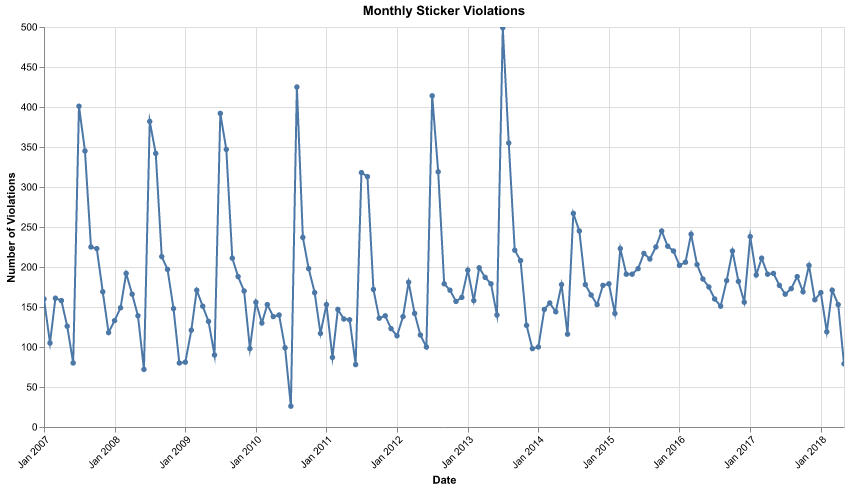
\includegraphics{ps2_answers_files/figure-pdf/cell-10-output-1.png}

2.2

\begin{Shaded}
\begin{Highlighting}[]
\CommentTok{\# Adding the price increase line at Feb 25, 2024. This is based on the data, where}
\CommentTok{\# we see that 02/25 is the first date of issue with the new code and 02/24 of the previous year}
\CommentTok{\# was the last day of issue using the old code.}
\NormalTok{base\_chart }\OperatorTok{=}\NormalTok{ alt.Chart(sticker\_violations\_dt).mark\_line(point}\OperatorTok{=}\VariableTok{True}\NormalTok{).encode(}
\NormalTok{    x}\OperatorTok{=}\NormalTok{alt.X(}\StringTok{\textquotesingle{}yearmonth(issue\_date):T\textquotesingle{}}\NormalTok{, }
\NormalTok{            title}\OperatorTok{=}\StringTok{\textquotesingle{}Date\textquotesingle{}}\NormalTok{,}
\NormalTok{            axis}\OperatorTok{=}\NormalTok{alt.Axis(}\BuiltInTok{format}\OperatorTok{=}\StringTok{\textquotesingle{}\%b \%Y\textquotesingle{}}\NormalTok{, labelAngle}\OperatorTok{={-}}\DecValTok{45}\NormalTok{, labelOverlap}\OperatorTok{=}\VariableTok{False}\NormalTok{)),}
\NormalTok{    y}\OperatorTok{=}\NormalTok{alt.Y(}\StringTok{\textquotesingle{}count:Q\textquotesingle{}}\NormalTok{, }
\NormalTok{            title}\OperatorTok{=}\StringTok{\textquotesingle{}Number of Violations\textquotesingle{}}\NormalTok{,}
\NormalTok{            scale}\OperatorTok{=}\NormalTok{alt.Scale(zero}\OperatorTok{=}\VariableTok{False}\NormalTok{))}
\NormalTok{)}

\CommentTok{\# Create a vertical line for Feb 25, 2012}
\NormalTok{vertical\_line }\OperatorTok{=}\NormalTok{ alt.Chart(pd.DataFrame(\{}\StringTok{\textquotesingle{}date\textquotesingle{}}\NormalTok{: [}\StringTok{\textquotesingle{}2012{-}02{-}25\textquotesingle{}}\NormalTok{]\})).mark\_rule(}
\NormalTok{    color}\OperatorTok{=}\StringTok{\textquotesingle{}red\textquotesingle{}}\NormalTok{,}
\NormalTok{    strokeWidth}\OperatorTok{=}\DecValTok{2}
\NormalTok{).encode(}
\NormalTok{    x}\OperatorTok{=}\StringTok{\textquotesingle{}yearmonth(date):T\textquotesingle{}}
\NormalTok{)}

\CommentTok{\# Create a label for the vertical line}
\NormalTok{label }\OperatorTok{=}\NormalTok{ alt.Chart(pd.DataFrame(\{}\StringTok{\textquotesingle{}date\textquotesingle{}}\NormalTok{: [}\StringTok{\textquotesingle{}2012{-}02{-}25\textquotesingle{}}\NormalTok{], }\StringTok{\textquotesingle{}label\textquotesingle{}}\NormalTok{: [}\StringTok{\textquotesingle{}Feb 25, 2012\textquotesingle{}}\NormalTok{]\})).mark\_text(}
\NormalTok{    align}\OperatorTok{=}\StringTok{\textquotesingle{}left\textquotesingle{}}\NormalTok{,}
\NormalTok{    baseline}\OperatorTok{=}\StringTok{\textquotesingle{}bottom\textquotesingle{}}\NormalTok{,}
\NormalTok{    dy}\OperatorTok{={-}}\DecValTok{150}  \CommentTok{\# Adjust this value to position the label vertically}
\NormalTok{).encode(}
\NormalTok{    x}\OperatorTok{=}\StringTok{\textquotesingle{}yearmonth(date):T\textquotesingle{}}\NormalTok{,}
\NormalTok{    text}\OperatorTok{=}\StringTok{\textquotesingle{}label\textquotesingle{}}
\NormalTok{)}

\CommentTok{\# Combine all elements}
\NormalTok{total\_sticker\_violations }\OperatorTok{=}\NormalTok{ (base\_chart }\OperatorTok{+}\NormalTok{ vertical\_line }\OperatorTok{+}\NormalTok{ label).properties(}
\NormalTok{    title}\OperatorTok{=}\StringTok{\textquotesingle{}Monthly Sticker Violations\textquotesingle{}}\NormalTok{,}
\NormalTok{    width}\OperatorTok{=}\DecValTok{800}\NormalTok{,}
\NormalTok{    height}\OperatorTok{=}\DecValTok{400}
\NormalTok{).interactive()}

\CommentTok{\# Display the chart}
\NormalTok{total\_sticker\_violations}
\end{Highlighting}
\end{Shaded}

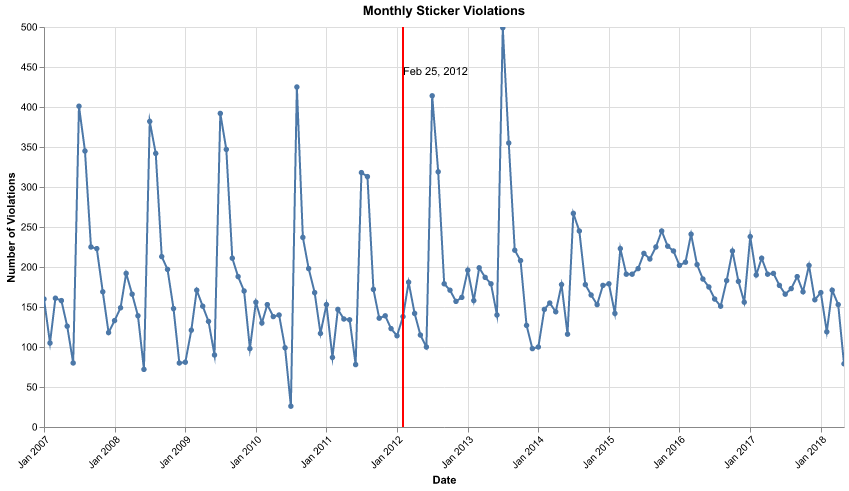
\includegraphics{ps2_answers_files/figure-pdf/cell-11-output-1.png}

I used the altair website guide in mark\_rule section and applied the
logic
https://altair-viz.github.io/gallery/bar\_chart\_with\_mean\_line.html

To add text to the line:
https://altair-viz.github.io/user\_guide/marks/text.html

2.3

\begin{Shaded}
\begin{Highlighting}[]
\CommentTok{\# Folter}
\NormalTok{sticker\_violations\_2011 }\OperatorTok{=}\NormalTok{ (}
\NormalTok{    sticker\_violations\_dt[sticker\_violations\_dt[}\StringTok{\textquotesingle{}issue\_date\textquotesingle{}}\NormalTok{].dt.year }\OperatorTok{==} \DecValTok{2011}\NormalTok{])}

\NormalTok{sticker\_violations\_2011[}\StringTok{\textquotesingle{}count\textquotesingle{}}\NormalTok{].}\BuiltInTok{sum}\NormalTok{()}
\end{Highlighting}
\end{Shaded}

\begin{verbatim}
1935
\end{verbatim}

There were 1935 observations (inluding code 0976170)
https://sparkbyexamples.com/pandas/pandas-filter-dataframe-rows-on-dates/\#:\textasciitilde:text=Filter\%20Rows\%20by\%20Dates\%20in\%20Pandas\%20DataFrame,-If\%20you\%20have\&text=to\_datetime()\%20you\%20can\%20just,data\%20type\%20of\%20all\%20columns.

\begin{Shaded}
\begin{Highlighting}[]
\NormalTok{prediction\_2011 }\OperatorTok{=} \DecValTok{1935} \OperatorTok{*} \DecValTok{100} \OperatorTok{*}\NormalTok{ (}\DecValTok{80}\NormalTok{)}
\BuiltInTok{print}\NormalTok{(}
    \SpecialStringTok{f\textquotesingle{}They should have predicted an increase of }\SpecialCharTok{\{}\NormalTok{prediction\_2011}\SpecialCharTok{\}}\SpecialStringTok{ USD in revenue\textquotesingle{}}\NormalTok{)}
\end{Highlighting}
\end{Shaded}

\begin{verbatim}
They should have predicted an increase of 15480000 USD in revenue
\end{verbatim}

They should have predicted an increase of 15,480,000 USD in revenue

2.4

\begin{Shaded}
\begin{Highlighting}[]
\NormalTok{sticker\_violations\_2013 }\OperatorTok{=}\NormalTok{ sticker\_violations\_monthly[}
\NormalTok{    sticker\_violations\_monthly[}\StringTok{\textquotesingle{}issue\_date\textquotesingle{}}\NormalTok{].dt.year }\OperatorTok{==} \DecValTok{2013}\NormalTok{]}

\NormalTok{issued\_2013 }\OperatorTok{=}\NormalTok{ sticker\_violations\_2013[}\StringTok{\textquotesingle{}ticket\_queue\textquotesingle{}}\NormalTok{].count()}

\BuiltInTok{print}\NormalTok{(issued\_2013)}
\CommentTok{\# Count paid tickets for 2013}
\NormalTok{paid\_2013 }\OperatorTok{=}\NormalTok{ sticker\_violations\_2013[sticker\_violations\_2013[}\StringTok{"ticket\_queue"}\NormalTok{]}
                                    \OperatorTok{==} \StringTok{"Paid"}\NormalTok{][}\StringTok{\textquotesingle{}ticket\_queue\textquotesingle{}}\NormalTok{].count()}

\CommentTok{\# Calculate ticket payment rate}
\NormalTok{ticket\_pay\_rate\_2013 }\OperatorTok{=}\NormalTok{ (paid\_2013 }\OperatorTok{/}\NormalTok{ issued\_2013) }\OperatorTok{*} \DecValTok{100}


\BuiltInTok{print}\NormalTok{(}\BuiltInTok{round}\NormalTok{(}\FloatTok{40.59213089209194}\NormalTok{,}\DecValTok{2}\NormalTok{))}
\end{Highlighting}
\end{Shaded}

\begin{verbatim}
2567
40.59
\end{verbatim}

The ticket pay rate is 40.59\% in 2013.

\begin{Shaded}
\begin{Highlighting}[]
\CommentTok{\# COunting the 2011 number of tickets issued}
\NormalTok{sticker\_violations\_2011 }\OperatorTok{=}\NormalTok{ sticker\_violations\_monthly[}
\NormalTok{    sticker\_violations\_monthly[}\StringTok{\textquotesingle{}issue\_date\textquotesingle{}}\NormalTok{].dt.year }\OperatorTok{==} \DecValTok{2011}\NormalTok{]}

\NormalTok{issued\_2011 }\OperatorTok{=}\NormalTok{ sticker\_violations\_2011[}\StringTok{\textquotesingle{}ticket\_queue\textquotesingle{}}\NormalTok{].count() }\OperatorTok{*} \DecValTok{100}
\BuiltInTok{print}\NormalTok{(}\SpecialStringTok{f\textquotesingle{}Tickets issued in 2011 were }\SpecialCharTok{\{}\NormalTok{issued\_2011}\SpecialCharTok{\}}\SpecialStringTok{\textquotesingle{}}\NormalTok{)}

\CommentTok{\# Count paid tickets for 2011}
\NormalTok{paid\_2011 }\OperatorTok{=}\NormalTok{ sticker\_violations\_2011[sticker\_violations\_2011[}\StringTok{"ticket\_queue"}\NormalTok{]}
                                    \OperatorTok{==} \StringTok{"Paid"}\NormalTok{][}\StringTok{\textquotesingle{}ticket\_queue\textquotesingle{}}\NormalTok{].count() }\OperatorTok{*} \DecValTok{100}

\CommentTok{\# Calculate ticket payment rate 2011}
\NormalTok{ticket\_pay\_rate\_2011 }\OperatorTok{=} \BuiltInTok{round}\NormalTok{((paid\_2011 }\OperatorTok{/}\NormalTok{ issued\_2011) }\OperatorTok{*} \DecValTok{100}\NormalTok{,}\DecValTok{2}\NormalTok{)}

\BuiltInTok{print}\NormalTok{(}\SpecialStringTok{f\textquotesingle{}The ticket pay rate in 2011 was }\SpecialCharTok{\{}\NormalTok{ticket\_pay\_rate\_2011}\SpecialCharTok{\}}\SpecialStringTok{\textquotesingle{}}\NormalTok{)}

\CommentTok{\# Change in repayment rate}
\NormalTok{repayment\_rate\_change }\OperatorTok{=} \BuiltInTok{round}\NormalTok{(ticket\_pay\_rate\_2011 }\OperatorTok{{-}}\NormalTok{ ticket\_pay\_rate\_2013,}\DecValTok{2}\NormalTok{)}
\BuiltInTok{print}\NormalTok{(}\SpecialStringTok{f\textquotesingle{}The change in repayment rater is }\SpecialCharTok{\{}\NormalTok{repayment\_rate\_change}\SpecialCharTok{\}}\SpecialStringTok{\textquotesingle{}}\NormalTok{)}

\NormalTok{revenue\_change\_2011\_2013 }\OperatorTok{=}\NormalTok{ (}\DecValTok{193500} \OperatorTok{*} \FloatTok{.4059} \OperatorTok{*} \DecValTok{200}\NormalTok{)}\OperatorTok{{-}}\NormalTok{(}\DecValTok{193500} \OperatorTok{*} \FloatTok{.5395} \OperatorTok{*} \DecValTok{120}\NormalTok{)}
\NormalTok{formatted\_revenue\_change\_2011\_2013 }\OperatorTok{=} \StringTok{\textquotesingle{}}\SpecialCharTok{\{:,.2f\}}\StringTok{\textquotesingle{}}\NormalTok{.}\BuiltInTok{format}\NormalTok{(revenue\_change\_2011\_2013)}
\NormalTok{revenue\_2013 }\OperatorTok{=} \DecValTok{193500} \OperatorTok{*} \FloatTok{.1336} \OperatorTok{*} \DecValTok{80}

\BuiltInTok{print}\NormalTok{(}\SpecialStringTok{f"The revenue change between 2011 and 2013 was an increase of $}\SpecialCharTok{\{}\NormalTok{formatted\_revenue\_change\_2011\_2013}\SpecialCharTok{\}}\SpecialStringTok{"}\NormalTok{)}
\BuiltInTok{print}\NormalTok{ (}\SpecialStringTok{f\textquotesingle{}The predicted revenue for 2013 would be }\SpecialCharTok{\{}\NormalTok{revenue\_2013}\SpecialCharTok{\}}\SpecialStringTok{ USD\textquotesingle{}}\NormalTok{)}
\end{Highlighting}
\end{Shaded}

\begin{verbatim}
Tickets issued in 2011 were 193500
The ticket pay rate in 2011 was 53.95
The change in repayment rater is 13.36
The revenue change between 2011 and 2013 was an increase of $3,181,140.00
The predicted revenue for 2013 would be 2068128.0 USD
\end{verbatim}

Tickets issued in 2011 were 193500 The ticket pay rate in 2011 was 53.95
The change in repayment rate is 13.36 The revenue change between 2011
and 2013 was an increase of \$3,181,140.00

2.5

\begin{Shaded}
\begin{Highlighting}[]
\CommentTok{\# Creating a loop function to get the repayment rates}
\NormalTok{years }\OperatorTok{=} \BuiltInTok{range}\NormalTok{(sticker\_violations\_monthly[}\StringTok{\textquotesingle{}issue\_date\textquotesingle{}}\NormalTok{].dt.year.}\BuiltInTok{min}\NormalTok{(), }
\NormalTok{              sticker\_violations\_monthly[}\StringTok{\textquotesingle{}issue\_date\textquotesingle{}}\NormalTok{].dt.year.}\BuiltInTok{max}\NormalTok{() }\OperatorTok{+} \DecValTok{1}\NormalTok{)}

\NormalTok{repayment\_rates }\OperatorTok{=}\NormalTok{ []}

\ControlFlowTok{for}\NormalTok{ year }\KeywordTok{in}\NormalTok{ years:}
\NormalTok{    sticker\_violations\_year }\OperatorTok{=}\NormalTok{ sticker\_violations\_monthly[}
\NormalTok{        sticker\_violations\_monthly[}\StringTok{\textquotesingle{}issue\_date\textquotesingle{}}\NormalTok{].dt.year }\OperatorTok{==}\NormalTok{ year]}
    
\NormalTok{    issued }\OperatorTok{=}\NormalTok{ sticker\_violations\_year[}\StringTok{\textquotesingle{}ticket\_queue\textquotesingle{}}\NormalTok{].count()}
\NormalTok{    paid }\OperatorTok{=}\NormalTok{ sticker\_violations\_year[sticker\_violations\_year[}\StringTok{"ticket\_queue"}\NormalTok{] }\OperatorTok{==} \StringTok{"Paid"}\NormalTok{][}\StringTok{\textquotesingle{}ticket\_queue\textquotesingle{}}\NormalTok{].count()}
    
\NormalTok{    repayment\_rate }\OperatorTok{=}\NormalTok{ (paid }\OperatorTok{/}\NormalTok{ issued) }\OperatorTok{*} \DecValTok{100} \ControlFlowTok{if}\NormalTok{ issued }\OperatorTok{\textgreater{}} \DecValTok{0} \ControlFlowTok{else} \DecValTok{0}
\NormalTok{    repayment\_rates.append(\{}\StringTok{\textquotesingle{}year\textquotesingle{}}\NormalTok{: year, }\StringTok{\textquotesingle{}repayment\_rate\textquotesingle{}}\NormalTok{: repayment\_rate\})}

\CommentTok{\# Create DataFrame from the results}
\NormalTok{df\_repayment }\OperatorTok{=}\NormalTok{ pd.DataFrame(repayment\_rates)}

\BuiltInTok{print}\NormalTok{(df\_repayment)}
\end{Highlighting}
\end{Shaded}

\begin{verbatim}
    year  repayment_rate
0   2007       55.085865
1   2008       57.885224
2   2009       53.113383
3   2010       51.987921
4   2011       53.953488
5   2012       48.220803
6   2013       40.592131
7   2014       38.419753
8   2015       40.616133
9   2016       40.768551
10  2017       37.012411
11  2018       20.144928
\end{verbatim}

\begin{Shaded}
\begin{Highlighting}[]
\CommentTok{\# Repayment rate chart}
\NormalTok{repayment\_rates\_chart }\OperatorTok{=}\NormalTok{ alt.Chart(df\_repayment).mark\_line(point}\OperatorTok{=}\VariableTok{True}\NormalTok{).encode(}
\NormalTok{    x}\OperatorTok{=}\NormalTok{alt.X(}\StringTok{\textquotesingle{}year:O\textquotesingle{}}\NormalTok{, title}\OperatorTok{=}\StringTok{\textquotesingle{}Year\textquotesingle{}}\NormalTok{),}
\NormalTok{    y}\OperatorTok{=}\NormalTok{alt.Y(}\StringTok{\textquotesingle{}repayment\_rate:Q\textquotesingle{}}\NormalTok{, title}\OperatorTok{=}\StringTok{\textquotesingle{}Repayment Rate (\%)\textquotesingle{}}\NormalTok{, scale}\OperatorTok{=}\NormalTok{alt.Scale(zero}\OperatorTok{=}\VariableTok{False}\NormalTok{))}
\NormalTok{).properties(}
\NormalTok{    title}\OperatorTok{=}\StringTok{\textquotesingle{}Repayment Rates for "Missing City Sticker" Tickets\textquotesingle{}}\NormalTok{,}
\NormalTok{    width}\OperatorTok{=}\DecValTok{800}\NormalTok{,}
\NormalTok{    height}\OperatorTok{=}\DecValTok{400}
\NormalTok{)}

\CommentTok{\# Add vertical line for policy introduction}
\NormalTok{policy\_line }\OperatorTok{=}\NormalTok{ alt.Chart(pd.DataFrame(\{}\StringTok{\textquotesingle{}year\textquotesingle{}}\NormalTok{: [}\DecValTok{2012}\NormalTok{]\})).mark\_rule(color}\OperatorTok{=}\StringTok{\textquotesingle{}red\textquotesingle{}}\NormalTok{).encode(}
\NormalTok{    x}\OperatorTok{=}\StringTok{\textquotesingle{}year:O\textquotesingle{}}
\NormalTok{)}

\CommentTok{\# Add text annotation for the policy line}
\NormalTok{policy\_text }\OperatorTok{=}\NormalTok{ alt.Chart(pd.DataFrame(\{}\StringTok{\textquotesingle{}year\textquotesingle{}}\NormalTok{: [}\DecValTok{2012}\NormalTok{], }\StringTok{\textquotesingle{}text\textquotesingle{}}\NormalTok{: [}\StringTok{\textquotesingle{}Price Increase Year\textquotesingle{}}\NormalTok{]\})).mark\_text(}
\NormalTok{    align}\OperatorTok{=}\StringTok{\textquotesingle{}right\textquotesingle{}}\NormalTok{,}
\NormalTok{    baseline}\OperatorTok{=}\StringTok{\textquotesingle{}top\textquotesingle{}}\NormalTok{,}
\NormalTok{    dx}\OperatorTok{=}\DecValTok{3}\NormalTok{,}
\NormalTok{    dy}\OperatorTok{=}\DecValTok{2}
\NormalTok{).encode(}
\NormalTok{    x}\OperatorTok{=}\StringTok{\textquotesingle{}year:O\textquotesingle{}}\NormalTok{,}
\NormalTok{    text}\OperatorTok{=}\StringTok{\textquotesingle{}text\textquotesingle{}}
\NormalTok{)}

\CommentTok{\# Combine the chart elements}
\NormalTok{repayment\_rates\_chart }\OperatorTok{=}\NormalTok{ (repayment\_rates\_chart }\OperatorTok{+}\NormalTok{ policy\_line }\OperatorTok{+}\NormalTok{ policy\_text).interactive()}

\CommentTok{\# Display the chart}
\NormalTok{repayment\_rates\_chart}
\end{Highlighting}
\end{Shaded}

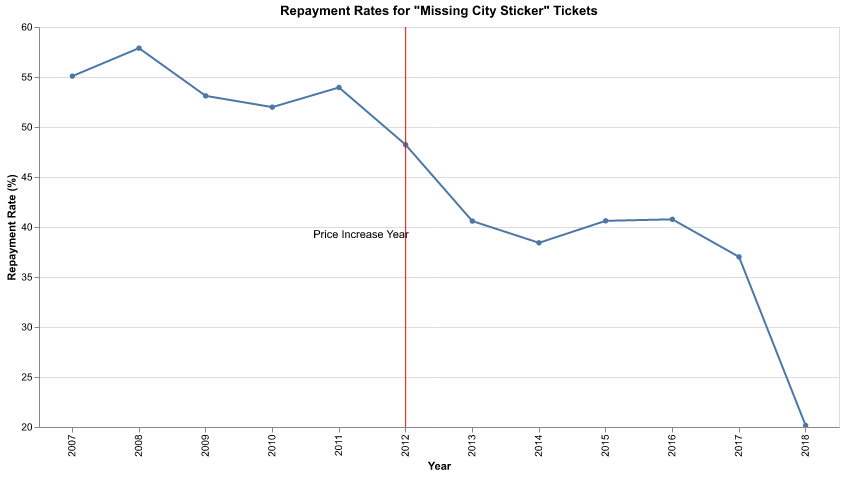
\includegraphics{ps2_answers_files/figure-pdf/cell-17-output-1.png}

To add the line on a specific date:
https://altair-viz.github.io/gallery/line\_chart\_with\_datum.html

To add text to the line:
https://altair-viz.github.io/user\_guide/marks/text.html The graph has a
clear downward trend, even before the price increase in 2012. However,
we do see that there seemed to be a sharper downward tren from
2012-2013, and then a sharper one from 2017 to 2018. From this, we can
glean that the city overestimated the revenue increase by a lot because
they did not account for the fact that people would probably have a hard
time repaying higher fines.

2.6

\begin{Shaded}
\begin{Highlighting}[]
\CommentTok{\# Calculate the issue count and repayment rates}
\NormalTok{total\_tickets }\OperatorTok{=}\NormalTok{ df[}\StringTok{\textquotesingle{}violation\_description\textquotesingle{}}\NormalTok{].value\_counts().reset\_index()}
\NormalTok{total\_tickets.columns }\OperatorTok{=}\NormalTok{ [}\StringTok{\textquotesingle{}violation\_description\textquotesingle{}}\NormalTok{, }\StringTok{\textquotesingle{}total\_tickets\textquotesingle{}}\NormalTok{]}

\CommentTok{\# Calculate repayment rates for each violation type}
\NormalTok{repayment\_rates\_by\_type }\OperatorTok{=}\NormalTok{ df.groupby(}\StringTok{\textquotesingle{}violation\_description\textquotesingle{}}\NormalTok{).}\BuiltInTok{apply}\NormalTok{(}
    \KeywordTok{lambda}\NormalTok{ x: (x[}\StringTok{\textquotesingle{}ticket\_queue\textquotesingle{}}\NormalTok{] }\OperatorTok{==} \StringTok{\textquotesingle{}Paid\textquotesingle{}}\NormalTok{).}\BuiltInTok{sum}\NormalTok{() }\OperatorTok{/} \BuiltInTok{len}\NormalTok{(x) }\OperatorTok{*} \DecValTok{100}
\NormalTok{).reset\_index()}
\NormalTok{repayment\_rates\_by\_type.columns }\OperatorTok{=}\NormalTok{ [}\StringTok{\textquotesingle{}violation\_description\textquotesingle{}}\NormalTok{, }\StringTok{\textquotesingle{}repayment\_rate\textquotesingle{}}\NormalTok{]}

\CommentTok{\# Merge the issue counts with repayment rates}
\NormalTok{result }\OperatorTok{=}\NormalTok{ pd.merge(total\_tickets, repayment\_rates\_by\_type, on}\OperatorTok{=}\StringTok{\textquotesingle{}violation\_description\textquotesingle{}}\NormalTok{)}

\CommentTok{\# Expected revenue}
\NormalTok{result[}\StringTok{\textquotesingle{}expected\_revenue\textquotesingle{}}\NormalTok{] }\OperatorTok{=}\NormalTok{ (result[}\StringTok{\textquotesingle{}total\_tickets\textquotesingle{}}\NormalTok{] }\OperatorTok{*}\NormalTok{ result[}\StringTok{\textquotesingle{}repayment\_rate\textquotesingle{}}\NormalTok{]) }\OperatorTok{/} \DecValTok{100}

\CommentTok{\# Round repayment\_rate and expected\_revenue for clarity}
\NormalTok{result[}\StringTok{\textquotesingle{}repayment\_rate\textquotesingle{}}\NormalTok{] }\OperatorTok{=}\NormalTok{ result[}\StringTok{\textquotesingle{}repayment\_rate\textquotesingle{}}\NormalTok{].}\BuiltInTok{round}\NormalTok{(}\DecValTok{2}\NormalTok{)}
\NormalTok{result[}\StringTok{\textquotesingle{}expected\_revenue\textquotesingle{}}\NormalTok{] }\OperatorTok{=}\NormalTok{ result[}\StringTok{\textquotesingle{}expected\_revenue\textquotesingle{}}\NormalTok{].}\BuiltInTok{round}\NormalTok{(}\DecValTok{2}\NormalTok{)}

\CommentTok{\# Sort by expected revenue in descending order and select top 10}
\NormalTok{top\_10 }\OperatorTok{=}\NormalTok{ result.sort\_values(}\StringTok{\textquotesingle{}expected\_revenue\textquotesingle{}}\NormalTok{, ascending}\OperatorTok{=}\VariableTok{False}\NormalTok{).head(}\DecValTok{10}\NormalTok{)}

\CommentTok{\# Display the top 10 table}
\BuiltInTok{print}\NormalTok{(}\StringTok{"Top 10 Violations by Expected Revenue:"}\NormalTok{)}
\BuiltInTok{print}\NormalTok{(top\_10[[}\StringTok{\textquotesingle{}violation\_description\textquotesingle{}}\NormalTok{, }\StringTok{\textquotesingle{}total\_tickets\textquotesingle{}}\NormalTok{, }\StringTok{\textquotesingle{}repayment\_rate\textquotesingle{}}\NormalTok{, }\StringTok{\textquotesingle{}expected\_revenue\textquotesingle{}}\NormalTok{]])}

\CommentTok{\# Find the violation with the highest expected revenue}
\NormalTok{highest\_revenue\_row }\OperatorTok{=}\NormalTok{ top\_10.loc[top\_10[}\StringTok{\textquotesingle{}expected\_revenue\textquotesingle{}}\NormalTok{].idxmax()]}
\NormalTok{highest\_revenue\_violation }\OperatorTok{=}\NormalTok{ highest\_revenue\_row[}\StringTok{\textquotesingle{}violation\_description\textquotesingle{}}\NormalTok{]}

\CommentTok{\# Print details}
\BuiltInTok{print}\NormalTok{(}\SpecialStringTok{f"}\CharTok{\textbackslash{}n}\SpecialStringTok{The violation with the highest expected revenue is: }\SpecialCharTok{\{}\NormalTok{highest\_revenue\_violation}\SpecialCharTok{\}}\SpecialStringTok{"}\NormalTok{)}
\BuiltInTok{print}\NormalTok{(}\SpecialStringTok{f"Details of this violation:}\CharTok{\textbackslash{}n}\SpecialCharTok{\{}\NormalTok{highest\_revenue\_row}\SpecialCharTok{\}}\SpecialStringTok{"}\NormalTok{)}
\end{Highlighting}
\end{Shaded}

\begin{verbatim}
Top 10 Violations by Expected Revenue:
                       violation_description  total_tickets  repayment_rate  \
0   EXPIRED PLATES OR TEMPORARY REGISTRATION          44811           60.44   
1                            STREET CLEANING          28712           81.16   
2                 RESIDENTIAL PERMIT PARKING          23683           74.23   
3   EXP. METER NON-CENTRAL BUSINESS DISTRICT          20600           79.29   
5                  EXPIRED METER OR OVERSTAY          18756           80.64   
4        PARKING/STANDING PROHIBITED ANYTIME          19753           70.58   
8                          RUSH HOUR PARKING          11965           77.04   
6              REAR AND FRONT PLATE REQUIRED          15829           53.05   
10   EXPIRED METER CENTRAL BUSINESS DISTRICT           9736           74.17   
11       NO STANDING/PARKING TIME RESTRICTED           8640           75.12   

    expected_revenue  
0            27082.0  
1            23303.0  
2            17579.0  
3            16334.0  
5            15124.0  
4            13942.0  
8             9218.0  
6             8397.0  
10            7221.0  
11            6490.0  

The violation with the highest expected revenue is: EXPIRED PLATES OR TEMPORARY REGISTRATION
Details of this violation:
violation_description    EXPIRED PLATES OR TEMPORARY REGISTRATION
total_tickets                                               44811
repayment_rate                                              60.44
expected_revenue                                          27082.0
Name: 0, dtype: object
\end{verbatim}

The violation that would earn the city the most money, given the numnber
of tickets issued and the repayment rate is EXPIRED PLATES OR TEMPORARY
REGISTRATION. This will lead to an expected revenue of \$2,708,200.0

\begin{Shaded}
\begin{Highlighting}[]
\NormalTok{top\_10\_chart }\OperatorTok{=}\NormalTok{ alt.Chart(top\_10).mark\_bar(color}\OperatorTok{=}\StringTok{\textquotesingle{}steelblue\textquotesingle{}}\NormalTok{).encode(}
\NormalTok{    x}\OperatorTok{=}\NormalTok{alt.X(}\StringTok{\textquotesingle{}violation\_description:N\textquotesingle{}}\NormalTok{,}
\NormalTok{            sort}\OperatorTok{=}\StringTok{\textquotesingle{}{-}y\textquotesingle{}}\NormalTok{,}
\NormalTok{            title}\OperatorTok{=}\StringTok{\textquotesingle{}Violation Type\textquotesingle{}}\NormalTok{,}
\NormalTok{            axis}\OperatorTok{=}\NormalTok{alt.Axis(}
\NormalTok{                labelAngle}\OperatorTok{={-}}\DecValTok{65}\NormalTok{,  }\CommentTok{\# Increased angle for better fit}
\NormalTok{                labelFontSize}\OperatorTok{=}\DecValTok{9}\NormalTok{,  }\CommentTok{\# Slightly reduced font size}
\NormalTok{                labelLimit}\OperatorTok{=}\DecValTok{300}\NormalTok{,  }\CommentTok{\# Increased label limit}
\NormalTok{                labelOverlap}\OperatorTok{=}\VariableTok{False}\NormalTok{,  }\CommentTok{\# Disable label overlap removal}
\NormalTok{                labelAlign}\OperatorTok{=}\StringTok{\textquotesingle{}right\textquotesingle{}}\NormalTok{,}
\NormalTok{                labelPadding}\OperatorTok{=}\DecValTok{4}
\NormalTok{            )}
\NormalTok{           ),  }
\NormalTok{    y}\OperatorTok{=}\NormalTok{alt.Y(}\StringTok{\textquotesingle{}expected\_revenue:Q\textquotesingle{}}\NormalTok{,}
\NormalTok{            title}\OperatorTok{=}\StringTok{\textquotesingle{}Expected Revenue ($)\textquotesingle{}}\NormalTok{),}
\NormalTok{).properties(}
\NormalTok{    width}\OperatorTok{=}\DecValTok{1200}\NormalTok{,  }\CommentTok{\# Increased width}
\NormalTok{    height}\OperatorTok{=}\DecValTok{600}\NormalTok{,  }\CommentTok{\# Increased height}
\NormalTok{    title}\OperatorTok{=}\StringTok{\textquotesingle{}Top 10 Violation Types by Expected Revenue\textquotesingle{}}
\NormalTok{).configure\_axis(}
\NormalTok{    titleFontSize}\OperatorTok{=}\DecValTok{14}\NormalTok{,}
\NormalTok{    labelFontSize}\OperatorTok{=}\DecValTok{9}  \CommentTok{\# Consistent font size for all labels}
\NormalTok{).configure\_view(}
\NormalTok{    strokeWidth}\OperatorTok{=}\DecValTok{0}  \CommentTok{\# Remove border around the chart}
\NormalTok{)}

\NormalTok{top\_10\_chart}
\end{Highlighting}
\end{Shaded}

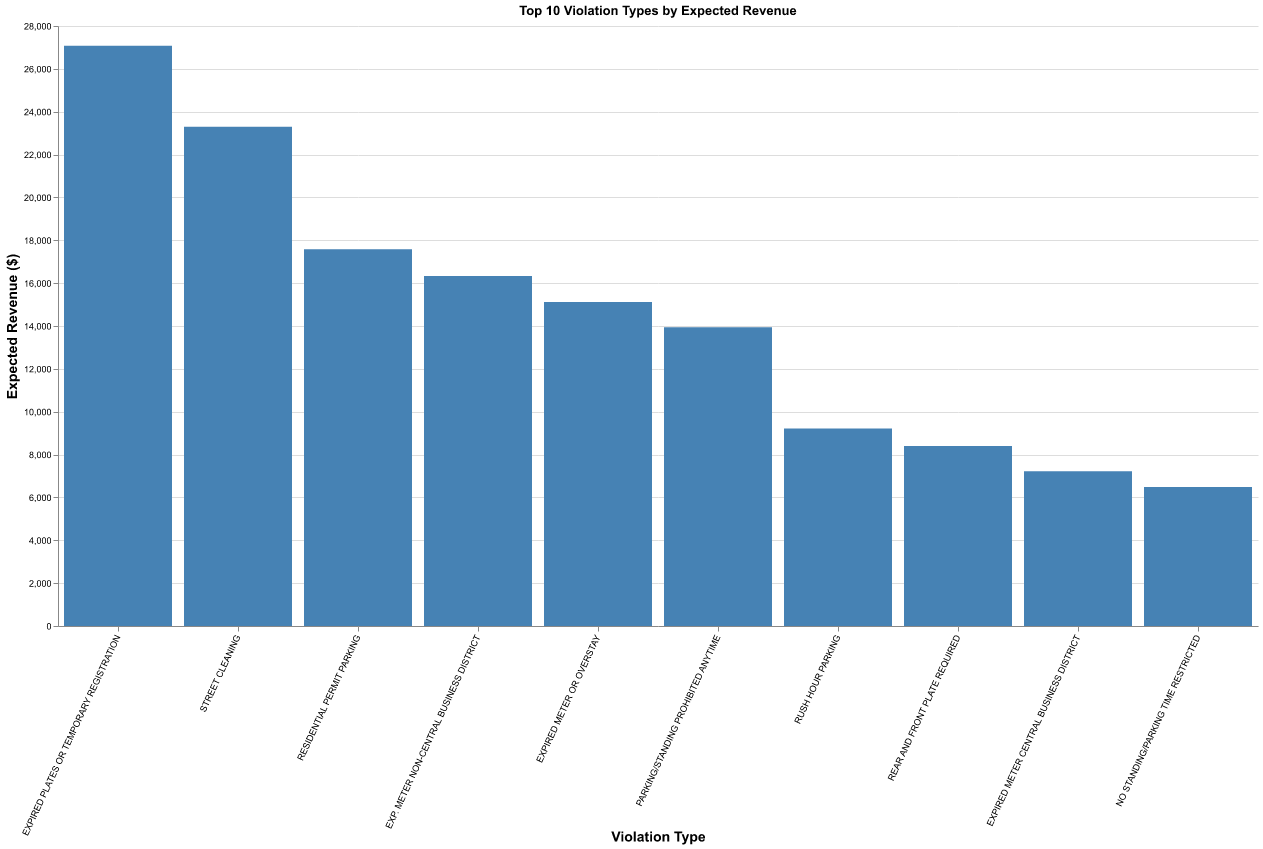
\includegraphics{ps2_answers_files/figure-pdf/cell-19-output-1.png}

\section{Part 3}\label{part-3}

3.1

\begin{Shaded}
\begin{Highlighting}[]
\NormalTok{merged\_sticker\_violations[}\StringTok{\textquotesingle{}is\_paid\textquotesingle{}}\NormalTok{] }\OperatorTok{=}\NormalTok{ merged\_sticker\_violations[}\StringTok{\textquotesingle{}ticket\_queue\textquotesingle{}}\NormalTok{] }\OperatorTok{==} \StringTok{\textquotesingle{}Paid\textquotesingle{}}

\CommentTok{\# Group by violation code and aggregate}
\NormalTok{violation\_summary }\OperatorTok{=}\NormalTok{ merged\_sticker\_violations.groupby(}\StringTok{\textquotesingle{}violation\_code\textquotesingle{}}\NormalTok{).agg(}
\NormalTok{    violation\_description}\OperatorTok{=}\NormalTok{(}\StringTok{\textquotesingle{}violation\_description\textquotesingle{}}\NormalTok{, }\StringTok{\textquotesingle{}first\textquotesingle{}}\NormalTok{),}
\NormalTok{    repayment\_rate}\OperatorTok{=}\NormalTok{(}\StringTok{\textquotesingle{}is\_paid\textquotesingle{}}\NormalTok{, }\StringTok{\textquotesingle{}mean\textquotesingle{}}\NormalTok{),}
\NormalTok{    avg\_fine\_level1}\OperatorTok{=}\NormalTok{(}\StringTok{\textquotesingle{}fine\_level1\_amount\textquotesingle{}}\NormalTok{, }\StringTok{\textquotesingle{}mean\textquotesingle{}}\NormalTok{),}
\NormalTok{    total\_tickets}\OperatorTok{=}\NormalTok{(}\StringTok{\textquotesingle{}violation\_description\textquotesingle{}}\NormalTok{, }\StringTok{\textquotesingle{}size\textquotesingle{}}\NormalTok{)}
\NormalTok{).reset\_index()}

\CommentTok{\# Sort by total tickets issued in descending order}
\NormalTok{sorted\_violation\_summary }\OperatorTok{=}\NormalTok{ violation\_summary.sort\_values(by}\OperatorTok{=}\StringTok{\textquotesingle{}total\_tickets\textquotesingle{}}\NormalTok{, ascending}\OperatorTok{=}\VariableTok{False}\NormalTok{).reset\_index()}

\CommentTok{\# Select only the desired columns}
\NormalTok{violation\_summary\_selected }\OperatorTok{=}\NormalTok{ sorted\_violation\_summary[[}\StringTok{\textquotesingle{}violation\_description\textquotesingle{}}\NormalTok{, }\StringTok{\textquotesingle{}repayment\_rate\textquotesingle{}}\NormalTok{, }\StringTok{\textquotesingle{}avg\_fine\_level1\textquotesingle{}}\NormalTok{]]}

\CommentTok{\# Display the top 5 most common violation descriptions}
\NormalTok{top\_5\_violation\_summary }\OperatorTok{=}\NormalTok{ violation\_summary\_selected.head(}\DecValTok{5}\NormalTok{)}
\BuiltInTok{print}\NormalTok{(top\_5\_violation\_summary)}
\end{Highlighting}
\end{Shaded}

\begin{verbatim}
                      violation_description  repayment_rate  avg_fine_level1
0  EXPIRED PLATES OR TEMPORARY REGISTRATION        0.604361        54.968869
1          STREET CLEANING OR SPECIAL EVENT        0.809083        53.583629
2       NO CITY STICKER OR IMPROPER DISPLAY        0.460770       165.552580
3                RESIDENTIAL PERMIT PARKING        0.742262        66.338302
4  EXP. METER NON-CENTRAL BUSINESS DISTRICT        0.792913        46.598058
\end{verbatim}

3.2

\begin{Shaded}
\begin{Highlighting}[]
\CommentTok{\# Selecting only tickets with that show up 100 or more times.}
\NormalTok{violation\_summary\_selected\_100 }\OperatorTok{=}\NormalTok{ sorted\_violation\_summary[sorted\_violation\_summary[}\StringTok{\textquotesingle{}total\_tickets\textquotesingle{}}\NormalTok{] }\OperatorTok{\textgreater{}=} \DecValTok{100}\NormalTok{]}

\CommentTok{\# Removing the highest fine}

\NormalTok{outlier\_fine }\OperatorTok{=}\NormalTok{ violation\_summary\_selected\_100[}\StringTok{\textquotesingle{}avg\_fine\_level1\textquotesingle{}}\NormalTok{].idxmax()}
\NormalTok{violation\_summary\_selected\_100 }\OperatorTok{=}\NormalTok{ violation\_summary\_selected\_100.drop(outlier\_fine)}

\CommentTok{\# Scatterplot}
\NormalTok{scatter\_fine\_repayment }\OperatorTok{=}\NormalTok{ alt.Chart(violation\_summary\_selected\_100).mark\_circle(color}\OperatorTok{=}\StringTok{\textquotesingle{}steelblue\textquotesingle{}}\NormalTok{).encode(}
\NormalTok{    x}\OperatorTok{=}\NormalTok{alt.X(}\StringTok{\textquotesingle{}avg\_fine\_level1:Q\textquotesingle{}}\NormalTok{, title}\OperatorTok{=}\StringTok{\textquotesingle{}Average Level 1 Fine ($)\textquotesingle{}}\NormalTok{),}
\NormalTok{    y}\OperatorTok{=}\NormalTok{alt.Y(}\StringTok{\textquotesingle{}repayment\_rate:Q\textquotesingle{}}\NormalTok{, title}\OperatorTok{=}\StringTok{\textquotesingle{}Repayment Rate\textquotesingle{}}\NormalTok{)}
\NormalTok{).properties(}
\NormalTok{    title}\OperatorTok{=}\StringTok{\textquotesingle{}Relationship Between Fine Amount and Repayment Rate\textquotesingle{}}
\NormalTok{)}

\NormalTok{scatter\_fine\_repayment.display()}

\CommentTok{\# BOXPLOT}
\NormalTok{box\_\_fine\_repayment }\OperatorTok{=}\NormalTok{ alt.Chart(violation\_summary\_selected\_100).mark\_boxplot().encode(}
\NormalTok{    x}\OperatorTok{=}\NormalTok{alt.X(}\StringTok{\textquotesingle{}avg\_fine\_level1:Q\textquotesingle{}}\NormalTok{, title}\OperatorTok{=}\StringTok{\textquotesingle{}Average Level 1 Fine ($)\textquotesingle{}}\NormalTok{, }\BuiltInTok{bin} \OperatorTok{=} \VariableTok{True}\NormalTok{),}
\NormalTok{    y}\OperatorTok{=}\NormalTok{alt.Y(}\StringTok{\textquotesingle{}repayment\_rate:Q\textquotesingle{}}\NormalTok{, title}\OperatorTok{=}\StringTok{\textquotesingle{}Repayment Rate\textquotesingle{}}\NormalTok{),}
\NormalTok{    tooltip}\OperatorTok{=}\NormalTok{[}\StringTok{\textquotesingle{}violation\_description\textquotesingle{}}\NormalTok{, }\StringTok{\textquotesingle{}total\_tickets\textquotesingle{}}\NormalTok{, }\StringTok{\textquotesingle{}avg\_fine\_level1\textquotesingle{}}\NormalTok{, }\StringTok{\textquotesingle{}repayment\_rate\textquotesingle{}}\NormalTok{]}
\NormalTok{).properties(}
\NormalTok{    title}\OperatorTok{=}\StringTok{\textquotesingle{}Relationship Between Fine Amount and Repayment Rate\textquotesingle{}}
\NormalTok{)}

\NormalTok{box\_\_fine\_repayment.display()}

\CommentTok{\# Bar graph}
\NormalTok{bar\_fine\_repayment }\OperatorTok{=}\NormalTok{ alt.Chart(violation\_summary\_selected\_100).mark\_bar().encode(}
\NormalTok{    x}\OperatorTok{=}\NormalTok{alt.X(}\StringTok{\textquotesingle{}avg\_fine\_level1:Q\textquotesingle{}}\NormalTok{, title}\OperatorTok{=}\StringTok{\textquotesingle{}Average Level 1 Fine ($)\textquotesingle{}}\NormalTok{),}
\NormalTok{    y}\OperatorTok{=}\NormalTok{alt.Y(}\StringTok{\textquotesingle{}repayment\_rate:Q\textquotesingle{}}\NormalTok{, title}\OperatorTok{=}\StringTok{\textquotesingle{}Repayment Rate\textquotesingle{}}\NormalTok{, scale}\OperatorTok{=}\NormalTok{alt.Scale(domain}\OperatorTok{=}\NormalTok{[}\FloatTok{0.1}\NormalTok{, }\FloatTok{0.9}\NormalTok{])),}
\NormalTok{    tooltip}\OperatorTok{=}\NormalTok{[}\StringTok{\textquotesingle{}violation\_description\textquotesingle{}}\NormalTok{, }\StringTok{\textquotesingle{}total\_tickets\textquotesingle{}}\NormalTok{, }\StringTok{\textquotesingle{}avg\_fine\_level1\textquotesingle{}}\NormalTok{, }\StringTok{\textquotesingle{}repayment\_rate\textquotesingle{}}\NormalTok{]}
\NormalTok{).properties(}
\NormalTok{    title}\OperatorTok{=}\StringTok{\textquotesingle{}Relationship Between Fine Amount and Repayment Rate\textquotesingle{}}
\NormalTok{)}

\NormalTok{bar\_fine\_repayment.display()}
\end{Highlighting}
\end{Shaded}

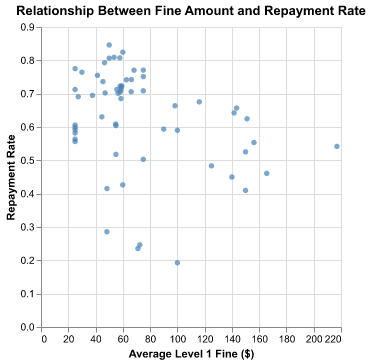
\includegraphics{ps2_answers_files/figure-pdf/cell-21-output-1.png}

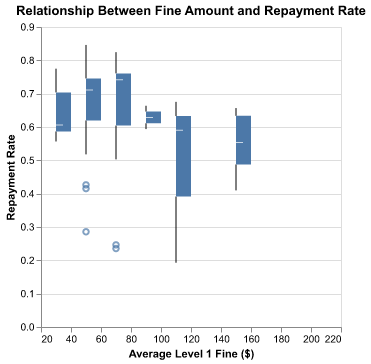
\includegraphics{ps2_answers_files/figure-pdf/cell-21-output-2.png}

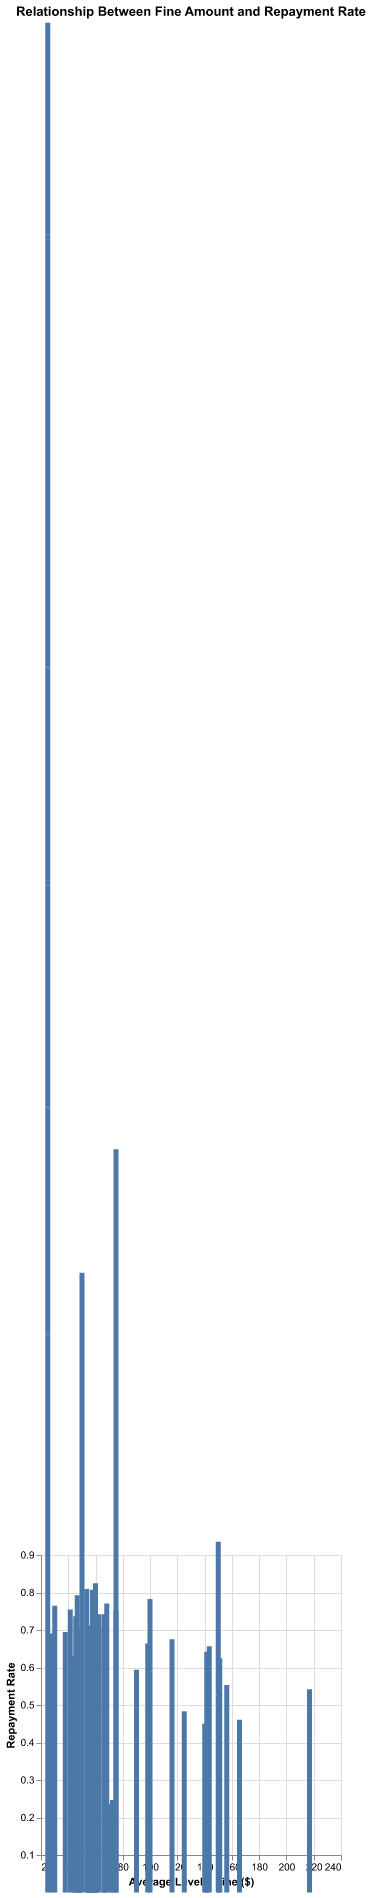
\includegraphics{ps2_answers_files/figure-pdf/cell-21-output-3.png}

Headline (scatter): Weak Negative Correlation Observed Between Fine
Amount and Repayment Rate Submessage(scatter): The scatterplot reveals a
weak negative correlation between average fine and repayment rate. As
the average fine increases, the repayment rate tends to decrease. Many
violation types have average fines clustered around the \$20-\$80 range,
with repayment rates varying significantly from 20\% to nearly 90\%.
Headline(box): Boxplot Provides Detailed Distribution Insights
Submessage(box): The boxplot offers a detailed view of data
distribution, showing medians, ranges, and outliers. Notably, fines set
at \$120 exhibit a wide range in repayment rates.We see that there
aren't observations past around \$150 fine level. Headline(bar): Bar
Graph Highlights Highest Repayment Rates Submessage(bar): The bar graph
clearly identifies violations with the highest repayment rates. However,
it does not effectively convey the variation per violation type or
illustrate the weak negative relationship as clearly as the
scatterplot.We also see that some fine levels have no observations.

3.2 Although it is more detailed, the averatge reader will have a hard
time understanding this, especialy if they're not that familiar with
statistics. That is why a scatterplot, thought it has less information,
is better for relaying information to the general public. At the very
least, you can provide the most salient pieces of data to them in a way
that is easily understood.

\section{Part 4}\label{part-4}

4.1

\begin{Shaded}
\begin{Highlighting}[]
\CommentTok{\# Checking if the fine doubles}
\NormalTok{df[}\StringTok{\textquotesingle{}fine\_doubles\textquotesingle{}}\NormalTok{] }\OperatorTok{=}\NormalTok{ df[}\StringTok{\textquotesingle{}fine\_level2\_amount\textquotesingle{}}\NormalTok{] }\OperatorTok{==}\NormalTok{ df[}\StringTok{\textquotesingle{}fine\_level1\_amount\textquotesingle{}}\NormalTok{] }\OperatorTok{*} \DecValTok{2}
\CommentTok{\# Checking if this is true for most of the data}
\NormalTok{double\_fine }\OperatorTok{=}\NormalTok{ df[}\StringTok{\textquotesingle{}fine\_doubles\textquotesingle{}}\NormalTok{].mean()}
\BuiltInTok{print}\NormalTok{(}\SpecialStringTok{f"We see that most fines do double }\SpecialCharTok{\{}\NormalTok{double\_fine}\SpecialCharTok{:.2\%\}}\SpecialStringTok{"}\NormalTok{)}
\end{Highlighting}
\end{Shaded}

\begin{verbatim}
We see that most fines do double 98.61%
\end{verbatim}

Not all violations double in price.

\begin{Shaded}
\begin{Highlighting}[]
\CommentTok{\# Filter for violations that do not double and drop NaN values}
\NormalTok{non\_double }\OperatorTok{=}\NormalTok{ df[df[}\StringTok{\textquotesingle{}fine\_level2\_amount\textquotesingle{}}\NormalTok{] }\OperatorTok{!=} \DecValTok{2} \OperatorTok{*}\NormalTok{ df[}\StringTok{\textquotesingle{}fine\_level1\_amount\textquotesingle{}}\NormalTok{]].dropna(subset}\OperatorTok{=}\NormalTok{[}\StringTok{\textquotesingle{}fine\_level1\_amount\textquotesingle{}}\NormalTok{, }\StringTok{\textquotesingle{}fine\_level2\_amount\textquotesingle{}}\NormalTok{])}

\CommentTok{\# Calculate fine increases for violations that do not double}
\NormalTok{non\_double[}\StringTok{\textquotesingle{}fine\_increase\textquotesingle{}}\NormalTok{] }\OperatorTok{=}\NormalTok{ non\_double[}\StringTok{\textquotesingle{}fine\_level2\_amount\textquotesingle{}}\NormalTok{] }\OperatorTok{{-}}\NormalTok{ non\_double[}\StringTok{\textquotesingle{}fine\_level1\_amount\textquotesingle{}}\NormalTok{]}

\CommentTok{\# Count citations for each violation description}
\NormalTok{non\_double\_counts }\OperatorTok{=}\NormalTok{ non\_double.groupby(}\StringTok{"violation\_description"}\NormalTok{).size().reset\_index(name}\OperatorTok{=}\StringTok{\textquotesingle{}citation\_count\textquotesingle{}}\NormalTok{)}

\CommentTok{\# Filter types with at least 100 citations}
\NormalTok{non\_double\_100 }\OperatorTok{=}\NormalTok{ non\_double\_counts[non\_double\_counts[}\StringTok{\textquotesingle{}citation\_count\textquotesingle{}}\NormalTok{] }\OperatorTok{\textgreater{}=} \DecValTok{100}\NormalTok{].reset\_index(drop}\OperatorTok{=}\VariableTok{True}\NormalTok{)}

\CommentTok{\# Merge the fine increase information back with the counts}
\NormalTok{non\_double\_fine\_increase }\OperatorTok{=}\NormalTok{ non\_double[non\_double[}\StringTok{\textquotesingle{}violation\_description\textquotesingle{}}\NormalTok{].isin(non\_double\_100[}\StringTok{\textquotesingle{}violation\_description\textquotesingle{}}\NormalTok{])]}


\NormalTok{non\_double\_fine\_increase }\OperatorTok{=}\NormalTok{ non\_double\_fine\_increase[[}\StringTok{\textquotesingle{}violation\_description\textquotesingle{}}\NormalTok{, }\StringTok{\textquotesingle{}fine\_increase\textquotesingle{}}\NormalTok{]].drop\_duplicates().reset\_index(drop}\OperatorTok{=}\VariableTok{True}\NormalTok{)}

\BuiltInTok{print}\NormalTok{(}\StringTok{"}\CharTok{\textbackslash{}n}\StringTok{ The fine increases for violations with at least 100 citations that do not double are:"}\NormalTok{)}
\BuiltInTok{print}\NormalTok{(non\_double\_fine\_increase)}
\end{Highlighting}
\end{Shaded}

\begin{verbatim}

 The fine increases for violations with at least 100 citations that do not double are:
                   violation_description  fine_increase
0                  DISABLED PARKING ZONE             50
1                    PARK OR BLOCK ALLEY            100
2   BLOCK ACCESS/ALLEY/DRIVEWAY/FIRELANE            100
3  SMOKED/TINTED WINDOWS PARKED/STANDING              0
\end{verbatim}

4.2 Attacking image (tip from Vitor) 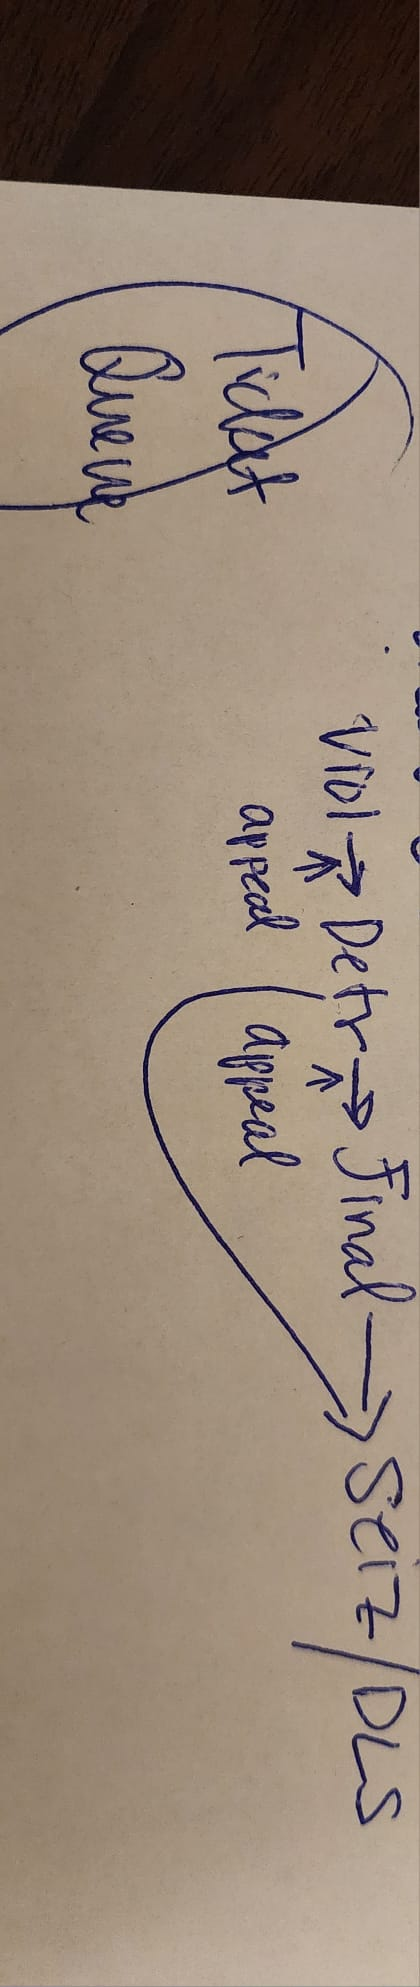
\includegraphics{ticket.jpg}
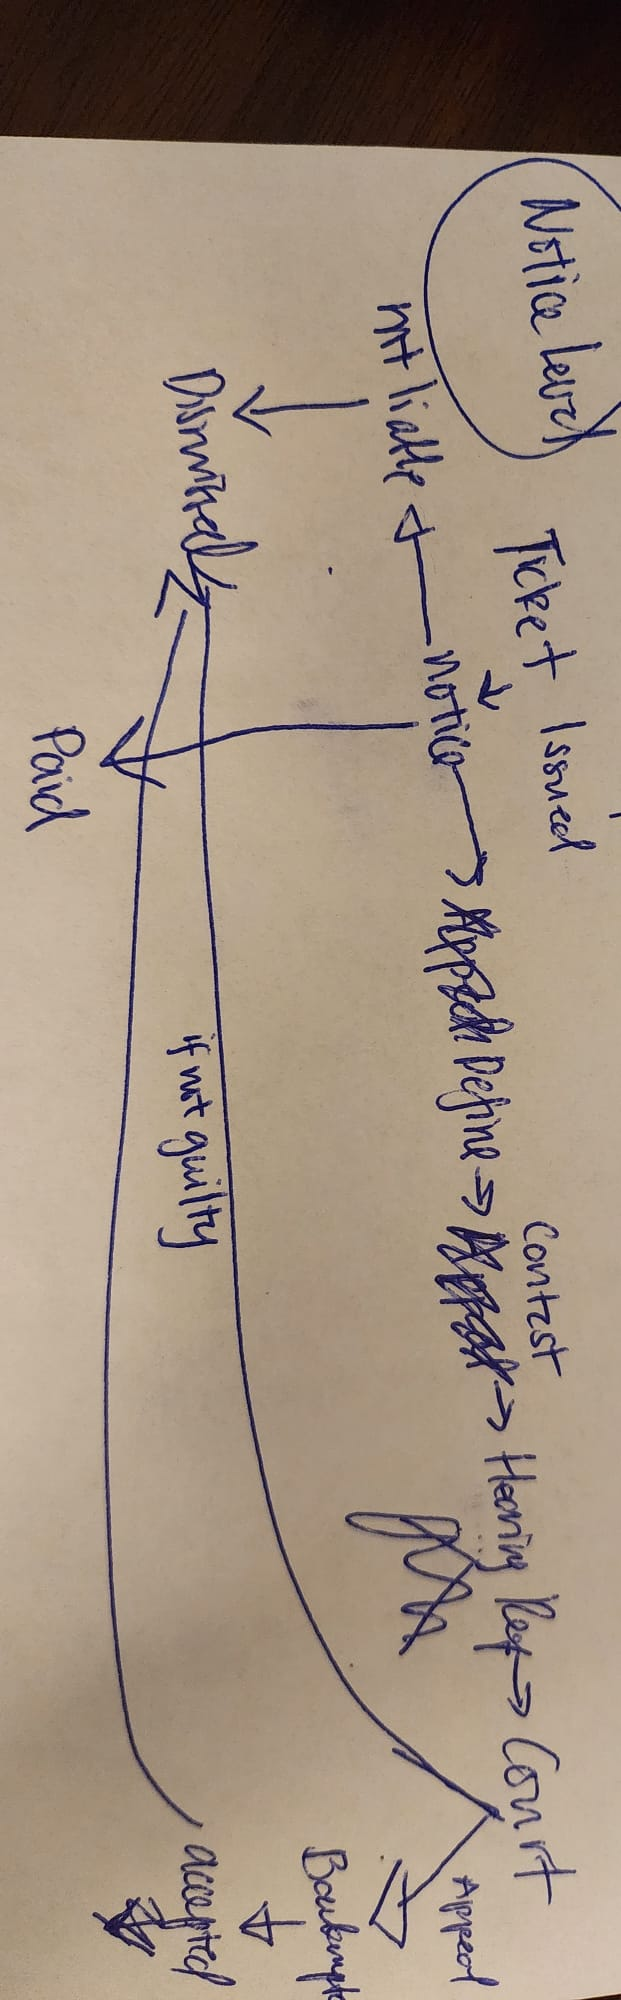
\includegraphics{notice_level.jpg}
https://www.chicago.gov/city/en/depts/fin/supp\_info/revenue/parking\_and\_red-lightnoticeinformation5/violation\_status.html

4.3 Making a scatterplot with labels

\begin{Shaded}
\begin{Highlighting}[]
\NormalTok{scatter\_labelled }\OperatorTok{=}\NormalTok{ alt.Chart(violation\_summary\_selected\_100).mark\_point().encode(}
\NormalTok{    x}\OperatorTok{=}\NormalTok{alt.X(}\StringTok{\textquotesingle{}avg\_fine\_level1:Q\textquotesingle{}}\NormalTok{, title}\OperatorTok{=}\StringTok{\textquotesingle{}Average Fine Level 1 ($)\textquotesingle{}}\NormalTok{),}
\NormalTok{    y}\OperatorTok{=}\NormalTok{alt.Y(}\StringTok{\textquotesingle{}repayment\_rate:Q\textquotesingle{}}\NormalTok{, title}\OperatorTok{=}\StringTok{\textquotesingle{}Repayment Rate\textquotesingle{}}\NormalTok{)}
\NormalTok{).properties(}
\NormalTok{    title}\OperatorTok{=}\StringTok{\textquotesingle{}Relationship Between Fine Amount and Repayment Rate\textquotesingle{}}
\NormalTok{)}

\NormalTok{scatter\_labelled.display()}

\NormalTok{text }\OperatorTok{=}\NormalTok{ scatter\_labelled.mark\_text(}
\NormalTok{    align}\OperatorTok{=}\StringTok{\textquotesingle{}center\textquotesingle{}}\NormalTok{,}
\NormalTok{    baseline}\OperatorTok{=}\StringTok{\textquotesingle{}middle\textquotesingle{}}
\NormalTok{).encode(}
\NormalTok{    text}\OperatorTok{=}\StringTok{\textquotesingle{}violation\_description:N\textquotesingle{}}
\NormalTok{)}

\NormalTok{scatter\_labelled }\OperatorTok{+}\NormalTok{ text}
\end{Highlighting}
\end{Shaded}

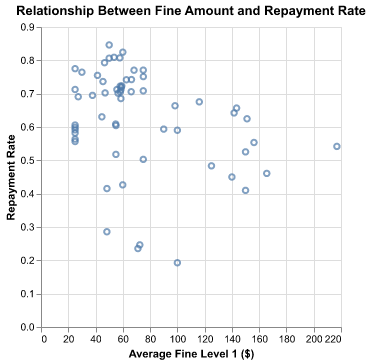
\includegraphics{ps2_answers_files/figure-pdf/cell-24-output-1.png}

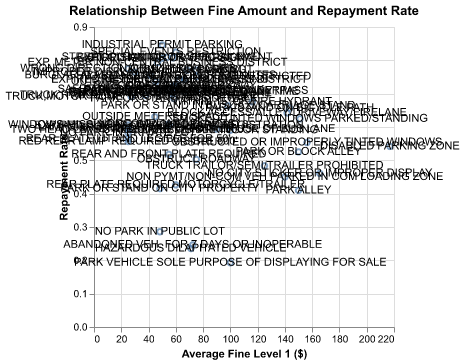
\includegraphics{ps2_answers_files/figure-pdf/cell-24-output-2.png}

Making a scatterplot with legend

\begin{Shaded}
\begin{Highlighting}[]
\NormalTok{scatter\_legend }\OperatorTok{=}\NormalTok{ alt.Chart(violation\_summary\_selected\_100).mark\_point(size}\OperatorTok{=}\DecValTok{60}\NormalTok{).encode(}
\NormalTok{    x}\OperatorTok{=}\NormalTok{alt.X(}\StringTok{\textquotesingle{}avg\_fine\_level1:Q\textquotesingle{}}\NormalTok{, title}\OperatorTok{=}\StringTok{\textquotesingle{}Average Fine Level 1 ($)\textquotesingle{}}\NormalTok{),}
\NormalTok{    y}\OperatorTok{=}\NormalTok{alt.Y(}\StringTok{\textquotesingle{}repayment\_rate:Q\textquotesingle{}}\NormalTok{, title}\OperatorTok{=}\StringTok{\textquotesingle{}Repayment Rate\textquotesingle{}}\NormalTok{),}
\NormalTok{    color}\OperatorTok{=}\NormalTok{alt.Color(}\StringTok{\textquotesingle{}violation\_description:N\textquotesingle{}}\NormalTok{, legend}\OperatorTok{=}\NormalTok{alt.Legend(title}\OperatorTok{=}\StringTok{\textquotesingle{}Violation Description\textquotesingle{}}\NormalTok{))  }
\NormalTok{).properties(}
\NormalTok{    title}\OperatorTok{=}\StringTok{\textquotesingle{}Relationship Between Fine Amount and Repayment Rate\textquotesingle{}}
\NormalTok{)}

\CommentTok{\# Display the scatter plot}
\NormalTok{scatter\_legend.display()}
\end{Highlighting}
\end{Shaded}

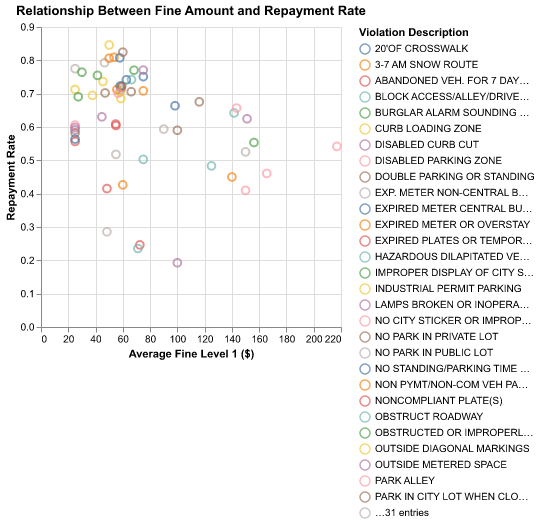
\includegraphics{ps2_answers_files/figure-pdf/cell-25-output-1.png}

Revising the plots

\begin{Shaded}
\begin{Highlighting}[]
\CommentTok{\# The top 10 violations are in the top\_10 df}
\BuiltInTok{print}\NormalTok{(top\_10)}
\CommentTok{\# Label the top 10 violations and mark others as \textquotesingle{}Other\textquotesingle{}}
\NormalTok{violation\_summary\_selected\_100[}\StringTok{\textquotesingle{}violation\_label\textquotesingle{}}\NormalTok{] }\OperatorTok{=}\NormalTok{ violation\_summary\_selected\_100[}\StringTok{\textquotesingle{}violation\_description\textquotesingle{}}\NormalTok{].where(}
\NormalTok{    violation\_summary\_selected\_100[}\StringTok{\textquotesingle{}violation\_description\textquotesingle{}}\NormalTok{].isin(top\_10[}\StringTok{\textquotesingle{}violation\_description\textquotesingle{}}\NormalTok{]),}
    \StringTok{\textquotesingle{}Other\textquotesingle{}}
\NormalTok{)}

\CommentTok{\# Create the scatter plot}
\NormalTok{scatter\_top\_10 }\OperatorTok{=}\NormalTok{ alt.Chart(violation\_summary\_selected\_100).mark\_point(size}\OperatorTok{=}\DecValTok{60}\NormalTok{).encode(}
\NormalTok{    x}\OperatorTok{=}\NormalTok{alt.X(}\StringTok{\textquotesingle{}avg\_fine\_level1:Q\textquotesingle{}}\NormalTok{, title}\OperatorTok{=}\StringTok{\textquotesingle{}Average Fine Level 1 ($)\textquotesingle{}}\NormalTok{),}
\NormalTok{    y}\OperatorTok{=}\NormalTok{alt.Y(}\StringTok{\textquotesingle{}repayment\_rate:Q\textquotesingle{}}\NormalTok{, title}\OperatorTok{=}\StringTok{\textquotesingle{}Repayment Rate\textquotesingle{}}\NormalTok{),}
\NormalTok{    color}\OperatorTok{=}\NormalTok{alt.Color(}\StringTok{\textquotesingle{}violation\_label:N\textquotesingle{}}\NormalTok{, legend}\OperatorTok{=}\NormalTok{alt.Legend(title}\OperatorTok{=}\StringTok{\textquotesingle{}Violation Description\textquotesingle{}}\NormalTok{))  }\CommentTok{\# Optional: add color encoding for labels}
\NormalTok{).properties(}
\NormalTok{    title}\OperatorTok{=}\StringTok{\textquotesingle{}Relationship Between Fine Amount and Repayment Rate\textquotesingle{}}
\NormalTok{)}

\CommentTok{\# Add ing labels}
\NormalTok{text }\OperatorTok{=}\NormalTok{ scatter\_top\_10.mark\_text(}
\NormalTok{    align}\OperatorTok{=}\StringTok{\textquotesingle{}left\textquotesingle{}}\NormalTok{,}
\NormalTok{    baseline}\OperatorTok{=}\StringTok{\textquotesingle{}middle\textquotesingle{}}\NormalTok{,}
\NormalTok{    dx}\OperatorTok{=}\DecValTok{7}
\NormalTok{).encode(}
\NormalTok{    text}\OperatorTok{=}\StringTok{\textquotesingle{}violation\_label:N\textquotesingle{}}  \CommentTok{\# Use the new \textquotesingle{}violation\_label\textquotesingle{} column for labels}
\NormalTok{)}

\CommentTok{\# Combine the scatter plot and text labels}
\NormalTok{scatter\_top\_10 }\OperatorTok{=}\NormalTok{ scatter\_top\_10 }\OperatorTok{+}\NormalTok{ text}

\CommentTok{\# Display the final chart}
\NormalTok{scatter\_top\_10.display()}
\end{Highlighting}
\end{Shaded}

\begin{verbatim}
                       violation_description  total_tickets  repayment_rate  \
0   EXPIRED PLATES OR TEMPORARY REGISTRATION          44811           60.44   
1                            STREET CLEANING          28712           81.16   
2                 RESIDENTIAL PERMIT PARKING          23683           74.23   
3   EXP. METER NON-CENTRAL BUSINESS DISTRICT          20600           79.29   
5                  EXPIRED METER OR OVERSTAY          18756           80.64   
4        PARKING/STANDING PROHIBITED ANYTIME          19753           70.58   
8                          RUSH HOUR PARKING          11965           77.04   
6              REAR AND FRONT PLATE REQUIRED          15829           53.05   
10   EXPIRED METER CENTRAL BUSINESS DISTRICT           9736           74.17   
11       NO STANDING/PARKING TIME RESTRICTED           8640           75.12   

    expected_revenue  
0            27082.0  
1            23303.0  
2            17579.0  
3            16334.0  
5            15124.0  
4            13942.0  
8             9218.0  
6             8397.0  
10            7221.0  
11            6490.0  
\end{verbatim}

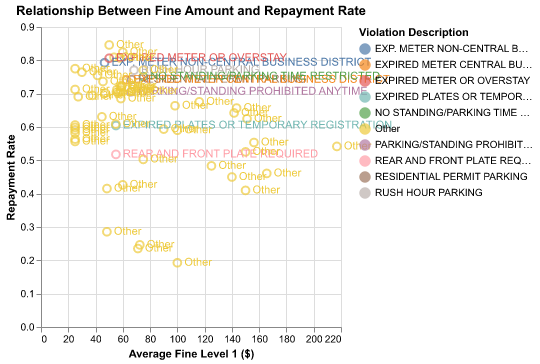
\includegraphics{ps2_answers_files/figure-pdf/cell-26-output-2.png}

Revising the plots (B)

\begin{Shaded}
\begin{Highlighting}[]
\CommentTok{\# Based on the top 10, we can group exp, park, sticker, and plate together.}
\NormalTok{unique\_violations }\OperatorTok{=}\NormalTok{ top\_10[}\StringTok{\textquotesingle{}violation\_description\textquotesingle{}}\NormalTok{].unique()}

\CommentTok{\# Convert to a list}
\NormalTok{unique\_violations\_list }\OperatorTok{=}\NormalTok{ unique\_violations.tolist()}

\NormalTok{unique\_violations\_df }\OperatorTok{=}\NormalTok{ pd.DataFrame(}
\NormalTok{    unique\_violations\_list, columns}\OperatorTok{=}\NormalTok{[}\StringTok{\textquotesingle{}unique\_values\textquotesingle{}}\NormalTok{])}


\KeywordTok{def}\NormalTok{ categorizing(description):}
    \ControlFlowTok{if} \StringTok{\textquotesingle{}EXP\textquotesingle{}} \KeywordTok{in}\NormalTok{ description:}
        \ControlFlowTok{return} \StringTok{\textquotesingle{}EXPIRATION\textquotesingle{}}
    \ControlFlowTok{elif} \StringTok{\textquotesingle{}STICKER\textquotesingle{}} \KeywordTok{in}\NormalTok{ description:}
        \ControlFlowTok{return} \StringTok{\textquotesingle{}STICKER\textquotesingle{}}
    \ControlFlowTok{elif} \StringTok{\textquotesingle{}PARK\textquotesingle{}} \KeywordTok{in}\NormalTok{ description:}
        \ControlFlowTok{return} \StringTok{\textquotesingle{}PARKING\textquotesingle{}}\NormalTok{,}
    \ControlFlowTok{else}\NormalTok{:}
        \ControlFlowTok{return} \StringTok{\textquotesingle{}OTHER\textquotesingle{}}

\CommentTok{\# Making a new column}
\NormalTok{violation\_summary\_selected\_100[}\StringTok{\textquotesingle{}violation\_category\textquotesingle{}}\NormalTok{] }\OperatorTok{=}\NormalTok{ violation\_summary\_selected\_100[}\StringTok{\textquotesingle{}violation\_description\textquotesingle{}}\NormalTok{].}\BuiltInTok{apply}\NormalTok{(}
\NormalTok{    categorizing)}

\CommentTok{\# Plotting}
\NormalTok{scatter\_categories }\OperatorTok{=}\NormalTok{ alt.Chart(violation\_summary\_selected\_100).mark\_point(filled}\OperatorTok{=}\VariableTok{True}\NormalTok{).encode(}
\NormalTok{    x}\OperatorTok{=}\NormalTok{alt.X(}\StringTok{\textquotesingle{}avg\_fine\_level1:Q\textquotesingle{}}\NormalTok{, title}\OperatorTok{=}\StringTok{\textquotesingle{}Average Fine Level 1 ($)\textquotesingle{}}\NormalTok{),}
\NormalTok{    y}\OperatorTok{=}\NormalTok{alt.Y(}\StringTok{\textquotesingle{}repayment\_rate:Q\textquotesingle{}}\NormalTok{, title}\OperatorTok{=}\StringTok{\textquotesingle{}Repayment Rate\textquotesingle{}}\NormalTok{),}
\NormalTok{    color}\OperatorTok{=}\NormalTok{alt.Color(}\StringTok{\textquotesingle{}violation\_category:N\textquotesingle{}}\NormalTok{, title}\OperatorTok{=}\StringTok{\textquotesingle{}Violation Category\textquotesingle{}}\NormalTok{,}
\NormalTok{                    scale}\OperatorTok{=}\NormalTok{alt.Scale(scheme}\OperatorTok{=}\StringTok{\textquotesingle{}category10\textquotesingle{}}\NormalTok{))}
\NormalTok{).properties(}
\NormalTok{    title}\OperatorTok{=}\StringTok{\textquotesingle{}Relationship Between Fine Amount and Repayment Rate\textquotesingle{}}
\NormalTok{)}

\NormalTok{scatter\_categories.display()}
\end{Highlighting}
\end{Shaded}

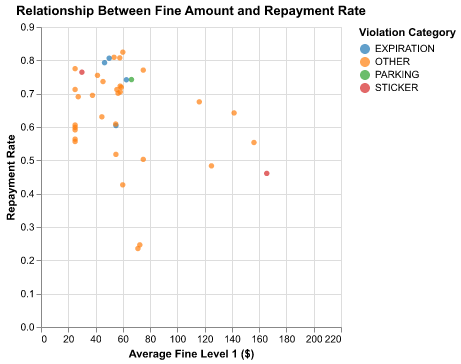
\includegraphics{ps2_answers_files/figure-pdf/cell-27-output-1.png}

\section{Extra Credit}\label{extra-credit}

\begin{Shaded}
\begin{Highlighting}[]
\CommentTok{\# getting patterns}
\NormalTok{patterns }\OperatorTok{=}\NormalTok{ df.groupby([}\StringTok{"violation\_code"}\NormalTok{, }\StringTok{"violation\_description"}\NormalTok{]).size().reset\_index(name}\OperatorTok{=}\StringTok{"count"}\NormalTok{)}

\CommentTok{\# Identify codes with multiple descriptions}
\NormalTok{multiple\_desc }\OperatorTok{=}\NormalTok{ patterns.groupby(}\StringTok{"violation\_code"}\NormalTok{).}\BuiltInTok{filter}\NormalTok{(}\KeywordTok{lambda}\NormalTok{ x: }\BuiltInTok{len}\NormalTok{(x) }\OperatorTok{\textgreater{}} \DecValTok{1}\NormalTok{)}

\CommentTok{\# Gettting the most common descriptions per code}
\NormalTok{common\_descriptions }\OperatorTok{=}\NormalTok{ multiple\_desc.loc[multiple\_desc.groupby(}\StringTok{"violation\_code"}\NormalTok{)[}\StringTok{"count"}\NormalTok{].idxmax()]}

\CommentTok{\# Making a dictionary for each one }
\NormalTok{common\_descriptions\_dict }\OperatorTok{=} \BuiltInTok{dict}\NormalTok{(}\BuiltInTok{zip}\NormalTok{(common\_descriptions[}\StringTok{"violation\_code"}\NormalTok{], common\_descriptions[}\StringTok{"violation\_description"}\NormalTok{]))}

\CommentTok{\# Filter the original dataframe for codes with multiple descriptions}
\NormalTok{df\_multi }\OperatorTok{=}\NormalTok{ df[df[}\StringTok{"violation\_code"}\NormalTok{].isin(common\_descriptions\_dict.keys())]}

\CommentTok{\# Add the major description column}
\NormalTok{df\_multi[}\StringTok{"major\_description"}\NormalTok{] }\OperatorTok{=}\NormalTok{ df\_multi[}\StringTok{"violation\_code"}\NormalTok{].}\BuiltInTok{map}\NormalTok{(common\_descriptions\_dict)}

\CommentTok{\# Get the top 3 codes by number of occurrences}
\NormalTok{top\_3\_codes }\OperatorTok{=}\NormalTok{ df\_multi[}\StringTok{"violation\_code"}\NormalTok{].value\_counts().head(}\DecValTok{3}\NormalTok{)}

\BuiltInTok{print}\NormalTok{(}\StringTok{"The top 3 violation codes with multiple descriptions 3:"}\NormalTok{)}
\BuiltInTok{print}\NormalTok{(top\_3\_codes)}

\BuiltInTok{print}\NormalTok{(df\_multi[[}\StringTok{"violation\_code"}\NormalTok{, }\StringTok{"violation\_description"}\NormalTok{, }\StringTok{"major\_description"}\NormalTok{]].head(}\DecValTok{10}\NormalTok{))}
\end{Highlighting}
\end{Shaded}

\begin{verbatim}
The top 3 violation codes with multiple descriptions 3:
violation_code
0964040B    32082
0976160A    16853
0976160B     3072
Name: count, dtype: int64
    violation_code             violation_description  \
6         0976160A     REAR AND FRONT PLATE REQUIRED   
16        0976160A     REAR AND FRONT PLATE REQUIRED   
17        0964200B             OUTSIDE METERED SPACE   
68        0964040B  STREET CLEANING OR SPECIAL EVENT   
75        0964040B  STREET CLEANING OR SPECIAL EVENT   
77        0964040B  STREET CLEANING OR SPECIAL EVENT   
80        0976160A     REAR AND FRONT PLATE REQUIRED   
94        0976160A     REAR AND FRONT PLATE REQUIRED   
96        0964040B  STREET CLEANING OR SPECIAL EVENT   
138       0976160A     REAR AND FRONT PLATE REQUIRED   

                 major_description  
6    REAR AND FRONT PLATE REQUIRED  
16   REAR AND FRONT PLATE REQUIRED  
17      PARK OUTSIDE METERED SPACE  
68                 STREET CLEANING  
75                 STREET CLEANING  
77                 STREET CLEANING  
80   REAR AND FRONT PLATE REQUIRED  
94   REAR AND FRONT PLATE REQUIRED  
96                 STREET CLEANING  
138  REAR AND FRONT PLATE REQUIRED  
\end{verbatim}




\end{document}
